% !TEX program = xelatex
% !BIB program = bibtex
% !TEX encoding = UTF-8
% 中文版必须用 xelatex 编译（xelatex -> bibtex -> xelatex -> xelatex），xeCJK 不支持 pdflatex。
\documentclass{article}
\usepackage{preprint}

\usepackage{amsmath,amssymb,amsthm,mathtools,bm}
\usepackage{booktabs}
\usepackage{multirow}
\usepackage{graphicx}
\usepackage{xcolor}
\usepackage{float}
\usepackage{tikz}
\usetikzlibrary{arrows.meta}
\usepackage{algorithm}
\usepackage[noend]{algpseudocode}
\floatname{algorithm}{算法}
\algrenewcommand\algorithmicrequire{\textbf{输入：}}
% 附录浮动体用 [!htbp] 让 LaTeX 自行填页，section 边界用 \FloatBarrier 拦住，避免 [H] 造成的整页空白
\usepackage[section]{placeins}
\renewcommand{\topfraction}{0.9}
\renewcommand{\bottomfraction}{0.8}
\renewcommand{\textfraction}{0.08}
\renewcommand{\floatpagefraction}{0.85}
\setcounter{topnumber}{4}
\setcounter{bottomnumber}{3}
\setcounter{totalnumber}{6}
% 浮动体页从顶部依次排列，不在浮动体之间均匀拉开空白
\makeatletter
\setlength{\@fptop}{0pt}
\setlength{\@fpsep}{\floatsep}
\setlength{\@fpbot}{0pt plus 1fil}
\makeatother

% hyperref 必须在浮动体相关的宏包之后加载，否则锚点重名
\usepackage{hyperref}
\usepackage{url}

% -------- 中文支持 --------
\usepackage{xeCJK}
% xeCJK loads fontspec, which resets the Latin fonts to Latin Modern; restore the Times/Helvetica pair of preprint.sty
\setmainfont{texgyretermes}[Extension = .otf, UprightFont = *-regular, BoldFont = *-bold, ItalicFont = *-italic, BoldItalicFont = *-bolditalic]
\setsansfont{texgyreheros}[Extension = .otf, UprightFont = *-regular, BoldFont = *-bold, ItalicFont = *-italic, BoldItalicFont = *-bolditalic]
\setCJKmainfont{SimSun}[BoldFont = SimHei, ItalicFont = KaiTi]
\setCJKsansfont{Microsoft YaHei}
\setCJKmonofont{FangSong}
\XeTeXlinebreaklocale "zh"
\XeTeXlinebreakskip = 0pt plus 1pt

\renewcommand{\proofname}{证明}
\renewcommand{\abstractname}{摘要}
\renewcommand{\figurename}{图}
\renewcommand{\tablename}{表}

% -------- 定理环境 --------
\theoremstyle{plain}
\newtheorem{theorem}{定理}[section]
\newtheorem{lemma}[theorem]{引理}
\newtheorem{corollary}[theorem]{推论}
\newtheorem{proposition}[theorem]{命题}
\theoremstyle{remark}
\newtheorem{remark}[theorem]{注}

% -------- 记号 --------
\newcommand{\Expl}{\mathrm{Expl}}
\newcommand{\Proj}{\Pi}
\newcommand{\simplex}{\Delta}
% 向量用小写粗体
\newcommand{\bx}{{\bm{x}}}
\newcommand{\by}{{\bm{y}}}
\newcommand{\bv}{{\bm{v}}}
\newcommand{\bw}{{\bm{w}}}
\newcommand{\bz}{{\bm{z}}}
\newcommand{\bu}{{\bm{u}}}
\newcommand{\bg}{{\bm{g}}}
\newcommand{\bq}{{\bm{q}}}
\newcommand{\br}{{\bm{r}}}
\newcommand{\be}{{\bm{e}}}
\newcommand{\brho}{{\bm{\rho}}}
\newcommand{\bell}{{\bm{\ell}}}
\newcommand{\aug}{\tilde{\bell}}
% 纳什策略、学习者的一步、自博弈顶点与自博弈权重
\newcommand{\xs}{\bx^{\star}}
\newcommand{\dx}{{\bm{s}}}
\newcommand{\esp}{\be_{\mathrm{sp}}}
\newcommand{\wsp}{w_{\mathrm{sp}}}
\newcommand{\coda}{CoDA}
\newcommand{\codar}{CoDA-R}
\newcommand{\rnad}{R-NaD-PPO}

% -------- 总览图（figures/overview.tex）的标签 --------
\newcommand{\ovLearner}{学习者}
\newcommand{\ovPool}{冻结对手池}
\newcommand{\ovOracle}{Oracle\\（可选）}
\newcommand{\ovWeightRule}{权重规则}
\newcommand{\ovPolicyUpdate}{策略更新}
\newcommand{\ovUpdateText}{针对自己与加权对手池\\做一步正则化更新}
\newcommand{\ovLossRates}{败率}
\newcommand{\ovWeights}{权重}
\newcommand{\ovGames}{对局}
\newcommand{\ovExploiter}{exploiter}
\newcommand{\ovSelfPlay}{自博弈}
\newcommand{\ovThreshold}{阈值}

\title{Coupled Dual-Adversarial Regularized Self-Play}

\author{YuLiang Xu}
\affiliation{Beijing No.~8 High School}
\email{ganggang2011@icloud.com}

\begin{document}

\maketitle

\begin{abstract}
在双人零和博弈中，当策略之间像剪刀石头布那样互相克制时，自博弈可能陷入循环。正则化自博弈消除了循环，训练的是单个网络，但这个网络只和自己对局，无法向外部对手学习。对手池方法让网络与一池对手对局，但它们保证收敛的是池上的混合，正在训练的那个网络没有保证。本文提出 Coupled Dual-Adversarial Regularized self-play（CoDA-R），让一个网络同时与自己和对手池对局。每次正则化的策略更新之前，一条闭式规则只把训练权重分给当前能击败该网络的池内对手，权重大小取决于它们的领先幅度。对精确算法，我们证明：无论对手如何入池或退出，所训练的策略本身都收敛到纳什均衡；并且只要池里有近似最佳响应，每一步都保证向均衡前进，前进量与 exploitability 的平方成正比。我们在近端策略优化（PPO）上实现 CoDA-R，并在五个不完美信息博弈上，以相同的预算与按同一协议调参的基线比较。CoDA-R 在三个博弈上取得单网络方法中最低的 exploitability，其中在 Goofspiel 与 Leduc 扑克上分别比正则化自博弈基线低 73\% 与 36\%；在一个博弈上与最好的方法持平，在一个博弈上排第二。受控实验表明，对手池能修补自博弈几乎走不到的漏洞，并使接近均衡的网络不再漂离。
\end{abstract}

% ----------------------------------------------------------------------
\section{引言}
% ----------------------------------------------------------------------

双人零和博弈是对抗性决策最基本的模型。棋类、扑克与即时战略游戏是它最直接的实例\citep{silver2018alphazero,brown2018libratus,vinyals2019alphastar,perolat2022stratego}，生成对抗网络与鲁棒优化的训练目标也是 min--max 问题\citep{goodfellow2014gan,daskalakis2018optimism}。这类问题自然的解概念是纳什策略，在对称博弈中，它是期望意义下没有任何对手能击败的策略。求纳什策略的常用办法是自博弈：让当前策略与自己或自己的历史版本对局，并用强化学习更新，既不需要人类数据，也不需要显式的对手模型。

自博弈有一个众所周知的失败模式。真实博弈中存在非传递的循环\citep{czarnecki2020spinning}：第一个策略击败第二个，第二个击败第三个，第三个又击败第一个。只针对当前策略更新的朴素自博弈会追着这些循环打转，无法收敛\citep{balduzzi2018mechanics,balduzzi2019openended}。现有的应对有两类。\emph{正则化自博弈}，如 Regularized Nash Dynamics（R-NaD）与 Magnetic Mirror Descent（MMD），惩罚策略与一个周期性移动的参考策略之间的距离。这把循环变成了收敛，而且保证落在正在训练的那个网络上\citep{perolat2021rnad,perolat2022stratego,sokota2023mmd}。但这个网络只和自己对局。脚本对手、早先的快照，以及 \emph{exploiter}（专门训练来击败当前策略的对手）都用不上，自博弈走不到的漏洞既不会被发现，也不会被修补\citep{openai2019dota,bansal2018emergent}。\emph{对手池方法}，如 Double Oracle、Policy-Space Response Oracles（PSRO）、prioritized fictitious self-play（PFSP）与联赛训练，让网络与一池这样的对手对局\citep{mcmahan2003doubleoracle,lanctot2017psro,vinyals2019alphastar}。它们若有保证，保证的也是池成员上的混合，或另外学习的平均网络，正在训练的网络没有保证。按胜率给池内对手加权的规则，如 PFSP 与 OpenAI Five 的采样器，则没有收敛证明。

\begin{figure}[t]
\begin{center}
% Overview figure shared by main.tex and main_zh.tex; the including file defines the \ov... label macros
\resizebox{0.98\linewidth}{!}{%
\begin{tikzpicture}[font=\footnotesize, >={Stealth[length=4pt]},
  box/.style={draw, rounded corners=2pt, align=center, inner sep=4pt, minimum height=9mm},
  note/.style={font=\scriptsize, align=center, inner sep=1.5pt}]
% -------- left panel: one step --------
\node[box, minimum width=22mm, fill=red!10] (learner) at (0,0) {\ovLearner\ $\bx_k$};
\node[box, text width=20mm, fill=blue!8] (pool) at (0,-2.2) {\ovPool\\$\by_1,\dots,\by_N$};
\node[box, densely dashed, minimum width=14mm] (oracle) at (-3.3,-2.2) {\ovOracle};
\node[box, text width=38mm, fill=black!6] (dual) at (4.6,-2.2) {\textbf{\ovWeightRule}\\$\bw=\Proj_{\simplex}\big(\esp+c\,\aug\big)$};
\node[box, text width=38mm, fill=black!6] (primal) at (4.6,0) {\textbf{\ovPolicyUpdate}\\\ovUpdateText};
\path[->] (learner) edge[loop above, looseness=5] node[note, above] {\ovSelfPlay} (learner);
\draw[<->] (learner) -- node[note, right] {\ovGames} (pool);
\draw[->] (pool) -- node[note, above] {\ovLossRates} node[note, below] {$\ell_i(\bx)$} (dual);
\draw[->] (dual) -- node[note, right] {\ovWeights\ $\bw$} (primal);
\draw[->] (primal) -- node[note, above] {$\bx_{k+1}$} (learner);
\draw[->, densely dashed] (oracle) -- node[note, above] {\ovExploiter} (pool);
\draw[->, densely dashed] (learner.west) -| (oracle.north);
% -------- right panel: the weight rule as a threshold, c = 2 and loss rates 0.9, 0.8, 0.5, 0.3 --------
\begin{scope}[shift={(8.3,-2.75)}, y=1.5cm]
\def\tauv{1.4667}
\draw[->] (0,0) -- (0,2.35);
\draw (0,0) -- (4.25,0);
% pool members: position, height c * loss rate, index, loss rate
\foreach \xpos/\h/\lab/\lr in {0.35/1.8/1/0.9, 1.1/1.6/2/0.8, 1.85/1.0/3/0.5, 2.6/0.6/4/0.3} {
  \fill[blue!12] (\xpos,0) rectangle (\xpos+0.5,\h);
  \draw[blue!45!black] (\xpos,0) rectangle (\xpos+0.5,\h);
  \node[note, below] at (\xpos+0.25,0) {$\by_{\lab}$};
  \node[note, below] at (\xpos+0.25,-0.22) {\lr};
}
% the part above the threshold is the weight
\foreach \xpos/\h/\wt in {0.35/1.8/0.33, 1.1/1.6/0.13} {
  \fill[red!65] (\xpos,\tauv) rectangle (\xpos+0.5,\h);
  \draw[blue!45!black] (\xpos,0) rectangle (\xpos+0.5,\h);
  \node[note, above] at (\xpos+0.25,\h) {\wt};
}
\node[note, above] at (2.1,1.0) {0};
\node[note, above] at (2.85,0.6) {0};
% self-play arm with height 1 + c / 2
\fill[black!10] (3.55,0) rectangle (4.05,2.0);
\fill[black!55] (3.55,\tauv) rectangle (4.05,2.0);
\draw[black!70] (3.55,0) rectangle (4.05,2.0);
\node[note, above] at (3.8,2.0) {0.53};
\node[note, below] at (3.8,0) {\ovSelfPlay};
\node[note, below] at (3.8,-0.22) {$\tfrac12$};
\node[note, below left] at (0.1,-0.22) {$\ell_i$};
% threshold and tie level
\draw[densely dashed] (0,\tauv) -- (4.25,\tauv);
\node[note, above] at (2.5,\tauv) {\ovThreshold};
\draw[dotted] (0,1.0) -- (3.4,1.0);
\node[note, left] at (0,1.0) {$\tfrac c2$};
\node[note, left] at (0,2.0) {$1+\tfrac c2$};
\node[note, left] at (0,\tauv) {$\tau$};
\end{scope}
\end{tikzpicture}%
}

\end{center}
\vspace{-4pt}
\caption{\codar{} 的一步。左：学习者与对手池、与自己对局；权重规则把败率变成权重，策略更新针对加权后的对手做一步正则化更新。右：权重规则的阈值形式（此处 $c=2$）。池成员 $i$ 的高度为 $c\,\ell_i$，自博弈的高度为 $1+\tfrac c2$；高出阈值 $\tau$ 的部分就是权重，所以打平或落后的成员权重恰为零。}
\label{fig:overview}
\end{figure}

本文要回答的问题是：一个网络能否在与开放的对手池对局的同时，自己就是那个收敛的对象。我们提出 Coupled Dual-Adversarial Regularized self-play（\codar{}），在每一步都精确计算时，答案是肯定的。\codar{} 维护一个策略，称为\emph{学习者}（learner），以及一个冻结的对手池，每一步分两部分（图~\ref{fig:overview}）。第一部分用一条闭式规则分配训练权重。池内对手只有在当前能击败学习者时才获得权重，领先越多权重越大；打平或落后的对手权重恰为零，剩下的权重归自博弈。第二部分让学习者针对自己与加权后的对手池做一步正则化更新，与正则化自博弈相同。权重的取法是使学习者的加权败率最大，相当于一个对抗者的对偶变量，方法的名字由此而来。这条规则只需要学习者对每个池成员的败率，而败率可以直接从训练对局中估计。因此任何能对局的智能体都可以成为池成员，包括脚本对手、其他架构的智能体，以及训练中由 \emph{oracle} 产生的 exploiter；而 PSRO 需要所有池成员两两之间的收益。

这两部分由一条不等式耦合在一起（定理~\ref{thm:energy}）。学习者的每一步移动、池持有的每一单位权重，都要由学习者到纳什策略的距离平方的下降来支付。这个距离有限，所以移动量与池权重都必须趋于零，而一个不再移动、池成员又不持有权重的策略，就是整个博弈的纳什策略。这个论证对任意的池内容、任意的池变化方式都成立。同一条不等式还说明了对手池带来什么：当池里有学习者的近似最佳响应时，每一步都使学习者向均衡前进，前进量与它的 exploitability 的平方成正比（定理~\ref{thm:oracle}）。本文的贡献如下。
\begin{itemize}
\item \textbf{算法。}\codar{} 让单个网络与自己、与一个由黑盒对手组成的开放对手池对局，权重规则是闭式的，不在各步之间保存任何状态。已有的池方法保证的是混合或时间平均，正则化自博弈不能接入外部对手；\codar{} 可以接入任何对手，并且保证落在所训练的策略本身。它包装的是未经修改的 PPO 学习器，只增加一个近端奖励项（\S\ref{sec:alg}、\S\ref{sec:impl}）。
\item \textbf{理论。}一条能量不等式把策略移动与池权重都记在到纳什均衡的距离上。由它得到：对任意的池变化序列，所训练的策略 last-iterate 收敛；池不再变化后有 $O(K^{-1/4})$ 的 last-iterate 速率；exploitability 有只含训练中可观测量的上界；所有的界都有带误差的版本（\S\ref{sec:theory}）。当池里有近似最佳响应时，它还给出每步进展关于 exploitability 平方的下界（定理~\ref{thm:oracle}）。
\item \textbf{实验。}在精确算法约 $10^8$ 条逐步记录中，没有一条不等式被违反。在 PPO 实现上，以相同的预算、所有基线按同一协议调参，\codar{} 的学习者在 Goofspiel(4)、Leduc 扑克与 3$\times$3 abrupt Dark Hex 上取得单网络中最低的末段 exploitability，在 abrupt Phantom Tic-Tac-Toe 上与 \rnad{} 持平。受控实验分离出对手池的贡献，以及权重规则与 PFSP 的区别（\S\ref{sec:exp}）。
\end{itemize}
权重规则的参考点固定在纯自博弈上。让参考点随训练移动的变体，是求解限制在池上的博弈时自然的设计，但它会卡在非均衡点上；\S\ref{sec:coda} 给出反例，并解释参考点为什么必须固定。

% ----------------------------------------------------------------------
\section{问题设定}
\label{sec:prelim}
% ----------------------------------------------------------------------

\subsection{博弈、败率与 exploitability}

考虑有限的双人零和博弈，每局开始前随机分配两个座位。这样博弈是\emph{对称}的，即两名玩家面对同一个决策问题；任何有限双人零和博弈都可以这样对称化。玩家有 $M$ 条纯策略（确定性策略），混合策略是纯策略上的概率分布，即概率单纯形
\[
X=\simplex_M:=\Big\{\bx\in\mathbb R^M:\ x_i\ge0,\ \textstyle\sum_ix_i=1\Big\}
\]
中的一个点。全文用 $\simplex_n$ 表示 $\mathbb R^n$ 中的概率单纯形。在完美回忆的序贯博弈中，混合策略等价于网络所表示的行为策略\citep{kuhn1953}，所以这种正规形无需额外假设就涵盖了扑克这样的博弈。此时 $M$ 非常大，但算法从不枚举纯策略，正规形只用于分析。

记 $\ell(\bx;\by)\in[0,1]$ 为策略 $\bx$ 对 $\by$ 的期望损失，结果按输记 1、赢记 0、平记 $\tfrac12$ 归一化。我们称它为\emph{败率}。由零和与对称性，$\ell(\bx;\by)+\ell(\by;\bx)=1$，故存在反对称矩阵 $S=-S^\top$ 使
\[
\ell(\bx;\by)=\tfrac12+\bx^\top S\by,\qquad \bx^\top S\bx=0 .
\]
特别地，任何策略与自己打平。策略的质量用\emph{可利用度}（exploitability）衡量，即最好的对手能击败它多少：
\[
\Expl(\bx):=\max_{\by\in X}\ell(\bx;\by)-\tfrac12=\max_j(S^\top \bx)_j\ \ge\ 0 .
\]
\emph{纳什策略} $\xs$ 是满足 $\Expl(\xs)=0$ 的策略。由 minimax 定理，它存在\citep{vonneumann1928}，并且
\begin{equation}
\xs\ \text{是纳什策略}\iff {\xs}^\top S\by\le0\ \ \forall \by\in X\iff \by^\top S\xs\ge0\ \ \forall \by\in X .
\label{eq:nash}
\end{equation}

\subsection{学习者、对手池与 oracle}
\label{sec:setting}

\emph{学习者}是唯一被训练的策略，$\bx_k$ 表示第 $k$ 步之后的学习者。除了与自己对局，它还可以与一个由冻结对手组成的\emph{对手池} $P=\{\by_1,\dots,\by_N\}\subset X$ 对局。池成员可以是任何能对局的智能体，例如学习者早先的快照、脚本对手、其他架构的智能体或 exploiter。成员是黑盒。算法只使用学习者与每个成员的对局结果，这些结果汇总为败率
\[
\ell_i(\bx):=\ell(\bx;\by_i)=\tfrac12+(S\by_i)^\top\bx ,\qquad i=1,\dots,N,
\]
每个都是 $\bx$ 的仿射函数，梯度为常向量 $S\by_i$。算法既不使用收益矩阵 $S$，也不使用池成员之间的收益。池可以在各步之间变化。\emph{oracle} 是任何这样的过程：给定冻结的学习者，返回一个意在击败它的对手，例如用强化学习训练的 exploiter，或者小博弈中的精确最佳响应；它的输出被加入对手池。

目标是学习者本身变得不可利用，即 $\Expl(\bx_k)\to0$。这是单个网络的 last-iterate 收敛，而不是多个网络上的混合的收敛。对手池从两方面服务于这个目标。它让自博弈永远产生不了的对手也能塑造学习者（\S\ref{sec:exp-mech}）；而且，池里有学习者的好的响应时，收敛会更快（定理~\ref{thm:oracle}）。

\subsection{投影}

全文中 $\|\cdot\|$ 表示欧氏范数，$\Proj_C$ 表示到闭凸集 $C$ 的欧氏投影。投影由\emph{投影不等式}刻画：
\begin{equation}
\bw=\Proj_C(\bv)\iff(\bv-\bw)^\top(\bu-\bw)\le0\quad\forall \bu\in C ,
\label{eq:obtuse}
\end{equation}
由它可以推出投影是单调且非扩张的\citep{bauschke2011convex}：对 $\bw=\Proj_C(\bz)$ 与 $\bw'=\Proj_C(\bz')$，在 \eqref{eq:obtuse} 中分别取 $\bu=\bw'$ 与 $\bu=\bw$ 再相加，得
\begin{equation}
(\bz-\bz')^\top(\bw-\bw')\ \ge\ \|\bw-\bw'\|^2\ \ge\ 0 .
\label{eq:monotone}
\end{equation}
到单纯形的投影有阈值形式 $\Proj_{\simplex_n}(\bz)_i=(z_i-\tau)^+$，其中 $(u)^+:=\max(u,0)$，阈值 $\tau$ 的取法是使各分量之和为 1；低于阈值的分量恰为零，$\tau$ 可以在 $O(n\log n)$ 时间内算出\citep{duchi2008projection}。单纯形的直径为 $D=\sqrt2$。除 minimax 定理与 Hartman--Stampacchia 定理外，本文的证明只用到投影不等式、配方法与极化恒等式 $\|\bu+\bv\|^2=\|\bu\|^2+\|\bv\|^2+2\bu^\top\bv$。表~\ref{tab:notation} 汇总了记号。

\begin{table}[t]
\caption{记号。}
\label{tab:notation}
\begin{center}
\small
\begin{tabular}{ll}
\toprule
记号 & 含义 \\
\midrule
$X=\simplex_M$ & $M$ 条纯策略上的混合策略 \\
$\ell(\bx;\by)$、$S$ & $\bx$ 对 $\by$ 的败率；$\ell(\bx;\by)=\tfrac12+\bx^\top S\by$，$S=-S^\top$ \\
$\Expl(\bx)$、$\xs$ & exploitability；纳什策略，$\Expl(\xs)=0$ \\
$\bx_k$、$\dx_k$ & 第 $k$ 步之后的学习者；它的一步 $\dx_k=\bx_{k+1}-\bx_k$ \\
$P=\{\by_1,\dots,\by_N\}$、$\ell_i(\bx)$ & 冻结对手组成的对手池；$\bx$ 对 $\by_i$ 的败率 \\
$\aug(\bx)$ & $(\ell_1(\bx),\dots,\ell_N(\bx),\tfrac12)$，补上自博弈一项的败率向量 \\
$\bw(\bx)$、$\bw_P$、$\wsp$ & 权重；它的池坐标；自博弈权重 \\
$\esp$ & $(0,\dots,0,1)$，全部权重在自博弈上 \\
$c$、$\eta$ & 对偶强度；近端强度 \\
$a$、$b$ & 池权重 $1-\wsp$；池压力 $\sum_iw_i(\ell_i-\tfrac12)$ \\
$\xi_k$、$\delta_k$、$\varepsilon$ & 败率估计、策略更新与 oracle 的误差 \\
\bottomrule
\end{tabular}
\end{center}
\end{table}

% ----------------------------------------------------------------------
\section{\codar{}}
\label{sec:alg}
% ----------------------------------------------------------------------

\begin{algorithm}[t]
\caption{\codar{} 的一步（精确形式；PPO 实现见 \S\ref{sec:impl}）}
\label{alg:codar}
\begin{algorithmic}[1]
\Require 学习者 $\bx_k$、对手池 $P=\{\by_1,\dots,\by_N\}$、对偶强度 $c>0$、近端强度 $\eta>0$
\State $\aug(\bx)\leftarrow\big(\ell_1(\bx),\dots,\ell_N(\bx),\tfrac12\big)$ \Comment{学习者的败率；自博弈恒为打平}
\State $\bw\leftarrow\Proj_{\simplex_{N+1}}\big(\esp+c\,\aug(\bx)\big)$ \Comment{权重规则（对偶侧）}
\State 让学习者与自己（系数 1）、与各 $\by_i$（系数 $w_i$）对局训练，并带惩罚项 $\tfrac\eta2\|\bx-\bx_k\|^2$ \Comment{策略更新（原侧）}
\State $\bx_k\leftarrow\bx_{k+1}$ \Comment{移动策略锚}
\State 可选：对 $\bx_{k+1}$ 调用 oracle，把返回的对手加入 $P$
\end{algorithmic}
\end{algorithm}

\codar{} 维护学习者 $\bx_k$ 与对手池 $P$。一步（算法~\ref{alg:codar}、图~\ref{fig:overview}）分两部分。\emph{权重规则}拿到学习者对每个池成员的败率，据此分配权重：当前能击败学习者的成员按领先幅度获得权重，其余成员恰为零，剩下的权重归自博弈。\emph{策略更新}再让学习者针对自己与加权后的对手池做一步正则化更新，并保持在上一个策略 $\bx_k$ 附近。权重是针对学习者选取的，是一个 min--max 问题中取最大的那个变量，所以我们也把权重规则称为对偶侧，把策略更新称为原侧。在 \S\ref{sec:theory} 分析的精确算法中，两部分都在新策略 $\bx_{k+1}$ 处取值，即这一步是隐式的；\S\ref{sec:impl} 说明 PPO 实现中所用的近似。

\subsection{权重规则}
\label{sec:dual}

自博弈被当作又一个对手，称为\emph{自博弈臂}。任何策略与自己打平，所以这个臂的败率恒为 $\tfrac12$，增广败率向量为
\[
\aug(\bx):=\big(\ell_1(\bx),\dots,\ell_N(\bx),\tfrac12\big)\in\mathbb R^{N+1}.
\]
记 $\esp:=(0,\dots,0,1)\in\simplex_{N+1}$ 为纯自博弈对应的权重向量，$c>0$ 为\emph{对偶强度}，它在训练中保持不变。给定策略 $\bx$，权重为
\begin{equation}
\bw(\bx):=\operatorname*{arg\,max}_{\bw\in\simplex_{N+1}}\Big[\bw^\top\aug(\bx)-\frac1{2c}\|\bw-\esp\|^2\Big]=\Proj_{\simplex_{N+1}}\big(\esp+c\,\aug(\bx)\big),
\label{eq:dual}
\end{equation}
第二个等号由配方法得到。方括号中的第一项把权重移向学习者输得最多的对手，第二项把权重拉回纯自博弈，$c$ 越大拉得越弱。我们称 $\esp$ 为\emph{对偶锚}，记 $\bw_P$ 为 $\bw$ 的池坐标（前 $N$ 个分量），$\wsp$ 为自博弈权重。

由投影的阈值形式，池成员的权重为 $w_i=(c\,\ell_i(\bx)-\tau)^+$，自博弈权重为 $\wsp=(1+\tfrac c2-\tau)^+$（图~\ref{fig:overview} 右）。与一个打平的成员相比，自博弈臂的高度多出 1，所以成员必须领先才能高出阈值。池里只有一个成员且它领先 $\mu$，即 $\ell_1(\bx)=\tfrac12+\mu$ 时，规则化为 $w_1=\operatorname{clip}(\tfrac{c\mu}2,0,1)$：不领先就没有权重，领先时权重与领先幅度成正比，斜率由 $c$ 决定。下面的引理给出一般性质，证明见附录~\ref{app:dual}。

\begin{lemma}[权重规则的性质]
\label{lem:dual}
(a) $\bw(\bx)=\esp$ 当且仅当 $\max_{i\in P}\ell_i(\bx)\le\tfrac12$。\\
(b) 持有权重的成员必定正在击败学习者：
\[
w_i(\bx)>0\ \Longrightarrow\ \ell_i(\bx)-\tfrac12\ \ge\ \frac{1-\wsp(\bx)+w_i(\bx)}{c}\ >\ 0 .
\]
(c) 若池中只有一个成员且 $\ell_1(\bx)=\tfrac12+\mu$，则 $w_1(\bx)=\operatorname{clip}(\tfrac{c\mu}{2},0,1)$。
\end{lemma}

由 (a)，没有成员击败学习者时，权重全部归自博弈，这一步就是一步正则化自博弈，即 R-NaD 与 MMD 共同的骨架；\codar{} 只在有对手击败学习者时才偏离正则化自博弈。由 (b)，持有权重的成员正在赢，权重越大的成员领先越多。有多个成员时，各权重共用一个阈值，没有逐成员的闭式。例如 $c=4$、两个成员的败率都是 0.9 时，$\esp+c\,\aug=(3.6,3.6,3)$，$\bw=(\tfrac12,\tfrac12,0)$，自博弈没有分到权重。

锚放在 $\esp$，是因为解处的正确权重事先就知道：没有对手能击败纳什策略，由 (a)，那里的权重就是 $\esp$。由于锚是固定的，$\bw(\bx)$ 是当前败率的连续闭式函数，不携带此前各步的任何状态。新的池成员不需要初始化，一个成员只要重新开始赢，就立刻重新获得权重。\S\ref{sec:coda} 说明，随训练移动的锚会失去收敛保证。

\subsection{策略更新}
\label{sec:primal}

固定上一个策略 $\bx_k$，它充当\emph{策略锚}，并固定\emph{近端强度} $\eta>0$。先假设对手是固定的：系数为 1 的自博弈对手 $\bar{\by}$，以及权重为 $\bw$ 的池成员。策略更新最小化加权败率与近端惩罚之和，
\begin{equation}
f_k(\bx):=\ell(\bx;\bar{\by})+\sum_{i\in P}w_i\,\ell_i(\bx)+\frac\eta2\|\bx-\bx_k\|^2,\qquad \bx\in X .
\label{eq:primal-obj}
\end{equation}
记 $A:=[S\by_1\cdots S\by_N]\in\mathbb R^{M\times N}$，前两项的梯度是常向量 $S\bar{\by}+A\bw_P$。由配方法，最小点是 $\Proj_X\big(\bx_k-\tfrac1\eta[S\bar{\by}+A\bw_P]\big)$，即从 $\bx_k$ 出发、步长为 $1/\eta$、使加权败率下降的一步投影更新。精确算法让对手在解本身处取值，$\bar{\by}=\bx_{k+1}$、$\bw=\bw(\bx_{k+1})$，于是更新为
\begin{equation}
\bx_{k+1}=\Proj_X\Big(\bx_k-\tfrac1\eta\big[S\bx_{k+1}+A\,\bw(\bx_{k+1})_P\big]\Big).
\label{eq:primal}
\end{equation}
未知量出现在等式两边，所以更新是隐式的。由投影不等式，\eqref{eq:primal} 等价于变分不等式
\begin{equation*}
\big\langle S\bx_{k+1}+A\,\bw(\bx_{k+1})_P+\eta(\bx_{k+1}-\bx_k),\ \bx'-\bx_{k+1}\big\rangle\ \ge\ 0\qquad\forall \bx'\in X ,
\tag{VI}
\label{eq:P}
\end{equation*}
它的三项分别是 \eqref{eq:primal-obj} 的三项在 $\bx_{k+1}$ 处的梯度：自博弈、对手池与近端惩罚。对任意 $\bx_k$ 与任意池，\eqref{eq:P} 恰有一个解（附录~\ref{app:unique} 的命题~\ref{prop:unique}）。后面所有的证明都是在 \eqref{eq:P} 中代入合适的测试点 $\bx'$。记
\[
\bv_{k+1}:=\bx_{k+1}+\textstyle\sum_iw_i(\bx_{k+1})\,\by_i,\qquad t_k:=2-\wsp(\bx_{k+1})\ \ge\ 1
\]
为合成对手及其总质量。于是 $S\bv_{k+1}$ 就是 \eqref{eq:P} 前两项之和，\eqref{eq:P} 说的是学习者对 $\bv_{k+1}$ 做了一步近端最佳响应。

隐式形式是必要的。分析需要权重与自博弈对手在同一点 $\bx_{k+1}$ 处取值（引理~\ref{lem:B}）。如果自博弈对手改用上一个策略 $\bx_k$，得到的显式更新会漂离均衡，在我们的矩阵博弈实验中它的 exploitability 停在 0.1 附近（附录图~\ref{fig:theory-nec}）。

\subsection{自博弈系数与对手采样}
\label{sec:share}

无论自博弈权重 $\wsp$ 是多少，自博弈在 \eqref{eq:P} 中的系数每一步都是 1，所以合成对手的质量总有 $t_k\ge1$。这个系数必须是一个正的常数。系数取 0 时，一旦池权重归零，\eqref{eq:P} 的前两项消失，每个 $\bx$ 都是不动点。系数取自博弈权重 $\wsp(\bx_{k+1})$ 时，自博弈项 $\wsp(\bx)S\bx$ 关于 $\bx$ 不再是反对称的，命题~\ref{prop:unique} 所依赖的单调性随之丧失。

系数描述的是训练目标，采样概率可以另外选取。实现可以按各臂上的任意分布 $\br$ 抽取对手，并给每一局乘上所属臂的重要性比，自博弈为 $1/r_{\mathrm{sp}}$，成员 $i$ 为 $w_i/r_i$；这样期望更新恰好是 \eqref{eq:P} 的更新。我们直接按权重抽取对手，$\br\propto(\bw_P,\wsp)$，并给自博弈臂设一个下限，以限制它的重要性比。若按系数的比例采样，$\br=(\bw_P,1)/t_k$，池在全部对局中的占比不超过 $(1-\wsp)/(2-\wsp)\le\tfrac12$，恰恰是持有权重的那些成员分到的对局太少，败率难以估准。

% ----------------------------------------------------------------------
\section{理论分析}
\label{sec:theory}
% ----------------------------------------------------------------------

本节分析精确算法：每一步都在 \S\ref{sec:prelim} 的正规形上精确求解 \eqref{eq:P}，池 $P_k$ 在各步之间可以任意变化。表~\ref{tab:guarantees} 汇总了结论。\S\ref{sec:energy} 证明所有结论依赖的那条不等式，\S\ref{sec:conv} 推出收敛、证书与速率，\S\ref{sec:oracle-rate} 定量给出 oracle 带来的增益，\S\ref{sec:inexact} 讨论混合策略与非精确步。

\begin{table}[t]
\caption{精确算法的保证。$K$ 为步数，$n$ 为池保持不变的最近步数。}
\label{tab:guarantees}
\begin{center}
\footnotesize
\setlength{\tabcolsep}{4pt}
\begin{tabular}{p{2.3cm}p{5.6cm}p{3.6cm}l}
\toprule
对象 & 保证 & 对池的条件 & 结论 \\
\midrule
学习者 $\bx_k$ & 收敛到纳什策略 & 任意的池序列 & 定理~\ref{thm:conv} \\
学习者 $\bx_k$ & $\min_{k<K}\Expl(\bx_{k+1})=O(K^{-1/2})$ & 任意的池序列 & 定理~\ref{thm:rate} \\
学习者 $\bx_K$ & $\Expl(\bx_K)=O(n^{-1/4})$ & $n$ 步内不变 & 定理~\ref{thm:rate} \\
学习者 $\bx_{k+1}$ & $\Expl(\bx_{k+1})\le\tfrac12a+\eta D\|\dx_k\|$，训练中可观测 & 任意池 & 定理~\ref{thm:cert} \\
学习者 $\bx_{k+1}$ & 到每个纳什策略的距离平方下降 $\tfrac{c}{4\eta}[\Expl(\bx_k)-\varepsilon]^{+2}$ & 含 $\bx_k$ 的 $\varepsilon$-最佳响应 & 定理~\ref{thm:oracle} \\
时间平均 $\bar{\bq}_K$ & $\Expl(\bar{\bq}_K)\le\eta/K$ & 任意的池序列 & 命题~\ref{prop:mix} \\
以上全部 & 相同的界加上误差项 & 非精确步 & 定理~\ref{thm:inexact} \\
\bottomrule
\end{tabular}
\end{center}
\end{table}

\subsection{能量不等式}
\label{sec:energy}

固定一步 $k$，简记 $\bx:=\bx_{k+1}$、$\bw:=\bw(\bx)$、$\bv:=\bv_{k+1}$；$\dx_k=\bx_{k+1}-\bx_k$ 是这一步的移动。用两个标量概括池在 $\bx$ 处的状态，即\emph{池权重} $a$ 与\emph{池压力} $b$：
\[
a(\bx):=1-\wsp=\textstyle\sum_{i\in P}w_i,\qquad
b(\bx):=\textstyle\sum_{i\in P}w_i\big(\ell_i(\bx)-\tfrac12\big).
\]
池压力是各成员的领先幅度按权重加权的和。由引理~\ref{lem:dual}(b)，持有权重的成员都有 $\ell_i>\tfrac12$，故 $b\ge0$。直接展开得到两个恒等式：
\begin{equation}
\bx^\top S\bv=\underbrace{\bx^\top S\bx}_{=0}+\textstyle\sum_iw_i\,\bx^\top S\by_i=b(\bx),\qquad
\bw^\top\aug(\bx)=\textstyle\sum_iw_i\ell_i(\bx)+\tfrac12\wsp=b(\bx)+\tfrac12 .
\label{eq:identities}
\end{equation}

第一个引理说，离开纯自博弈是有代价的。权重最大化的是加权败率减去到 $\esp$ 的距离的惩罚，所以池只有在成员当前赢得足够多时才能持有权重。

\begin{lemma}[池权重由当前的领先支撑]
\label{lem:A}
\[
b(\bx)\ \ge\ \frac1c\,\|\bw(\bx)-\esp\|^2 .
\]
\end{lemma}
\textit{证明。}$\bw=\Proj_\simplex(\esp+c\aug)$。在投影不等式 \eqref{eq:obtuse} 中取 $\bu=\esp\in\simplex$：
\[
\big(\esp+c\aug-\bw\big)^\top(\esp-\bw)\le0
\iff\|\esp-\bw\|^2+c\,\aug^\top(\esp-\bw)\le0 .
\]
由 \eqref{eq:identities}，$\aug^\top \esp=\tfrac12$，$\aug^\top \bw=b+\tfrac12$，故 $\aug^\top(\esp-\bw)=-b$。于是 $\|\bw-\esp\|^2\le c\,b$。\hfill$\blacksquare$

换句话说，池能持有多少权重，取决于它当前击败学习者多少；只是打平的池（$b=0$）不持有任何权重。

第二个引理把池压力变成移动。面对合成对手 $\bv$，学习者的超额损失是 $b$，而纳什策略的超额损失不超过零。因此朝 $\xs$ 移动至少能使 \eqref{eq:P} 中的损失项下降 $b$；而 \eqref{eq:P} 说的是没有任何可行方向能使整个目标下降，所以这个差额必须由近端项补上。

\begin{lemma}[池压力由朝均衡的进展支付]
\label{lem:B}
对任一纳什策略 $\xs$，
\[
\eta\,\dx_k^\top(\xs-\bx_{k+1})\ \ge\ b(\bx_{k+1}).
\]
\end{lemma}
\textit{证明。}在 \eqref{eq:P} 中取 $\bx'=\xs$，并把前两项合并为 $S\bv$：
\[
\langle S\bv,\,\xs-\bx\rangle+\eta\,\dx_k^\top(\xs-\bx)\ge0,\qquad
\langle S\bv,\,\xs-\bx\rangle={\xs}^\top S\bv-\bx^\top S\bv={\xs}^\top S\bv-b .
\]
$\bv=\bx+\sum_iw_i\by_i$ 是 $X$ 中若干点的非负组合，由 \eqref{eq:nash}，每一项都满足 ${\xs}^\top S\bz\le0$，故 ${\xs}^\top S\bv\le0$。于是 $\eta\,\dx_k^\top(\xs-\bx)\ge b-{\xs}^\top S\bv\ge b$。\hfill$\blacksquare$

\begin{theorem}[能量不等式]
\label{thm:energy}
对任意一步 $k$、任意池 $P_k$ 与任一纳什策略 $\xs$，
\begin{equation}
\|\bx_{k+1}-\xs\|^2+\|\bx_{k+1}-\bx_k\|^2+\frac{2}{c\eta}\|\bw(\bx_{k+1})-\esp\|^2\ \le\ \|\bx_k-\xs\|^2 .
\label{eq:energy}
\end{equation}
\end{theorem}
\textit{证明。}由极化恒等式，
\[
\|\bx_k-\xs\|^2=\|\dx_k\|^2+\|\bx_{k+1}-\xs\|^2+2\,\dx_k^\top(\xs-\bx_{k+1}) ,
\]
对交叉项先用引理~\ref{lem:B}，再用引理~\ref{lem:A}，
\[
2\,\dx_k^\top(\xs-\bx_{k+1})\ \ge\ \tfrac2\eta\,b(\bx_{k+1})\ \ge\ \tfrac{2}{c\eta}\|\bw(\bx_{k+1})-\esp\|^2 .\eqno\blacksquare
\]

到纳什策略的距离平方相当于一笔预算。\eqref{eq:energy} 的右端是这一步之前的预算；左端是这一步之后的预算，加上这一步的两项支出，即策略的移动与池持有的权重。预算不超过 $D^2=2$，它限制了整个训练过程中的总支出。

\begin{corollary}[移动量与池权重可和]
\label{cor:sum}
对 \eqref{eq:energy} 在 $k<K$ 上求和，
\[
\textstyle\sum_{k<K}\|\dx_k\|^2\le\|\bx_0-\xs\|^2\le2,\qquad
\sum_{k<K}\|\bw(\bx_{k+1})-\esp\|^2\le\tfrac{c\eta}2\|\bx_0-\xs\|^2\le c\eta ,
\]
从而 $\dx_k\to0$，$\bw(\bx_{k+1})\to \esp$，$a(\bx_{k+1})\le\|\bw(\bx_{k+1})-\esp\|\to0$。不等式 \eqref{eq:energy} 只涉及 $\bx_k$、$\bx_{k+1}$、$\bw(\bx_{k+1})$ 与整个博弈的纳什策略 $\xs$，所以在各步之间增删池成员（包括 oracle 的全部入池）不改变任何一步的这条不等式，上述结论在整个训练过程中成立。
\end{corollary}

\subsection{收敛、证书与速率}
\label{sec:conv}

我们把只含训练中可观测量的 exploitability 上界称为\emph{证书}。

\begin{theorem}[两条证书]
\label{thm:cert}
记 $D=\sqrt2$。(i) 学习者的全博弈证书：
\[
\Expl(\bx_{k+1})\ \le\ \tfrac12a(\bx_{k+1})-b(\bx_{k+1})+\eta D\|\dx_k\|\ \le\ \tfrac12a(\bx_{k+1})+\eta D\|\dx_k\| .
\]
(ii) 池内证书：
\[
\Big[\max_{i\in P}\ell_i(\bx_{k+1})-\tfrac12\Big]^+\ \le\ \frac{\sqrt2}{c}\,\|\bw(\bx_{k+1})-\esp\|+\eta D\|\dx_k\| .
\]
\end{theorem}
证明（附录~\ref{app:cert}）在 \eqref{eq:P} 中取 $\bx_{k+1}$ 的一个最佳响应作为测试点。朝它移动恰好使自博弈项下降 $\Expl(\bx_{k+1})$，所以池项与近端项必须补上这一部分，而这两项都被可观测量控制：池权重 $a$、到纯自博弈的距离 $\|\bw-\esp\|$，以及这一步的移动量 $\|\dx_k\|$。

\begin{theorem}[学习者收敛到纳什策略]
\label{thm:conv}
对精确步与任意的池 $P_k$，$\Expl(\bx_k)\to0$，且整个序列 $\bx_k$ 收敛到一个纳什策略。
\end{theorem}
证明见附录~\ref{app:conv}。推论~\ref{cor:sum} 给出 $a\to0$ 与 $\|\dx_k\|\to0$，所以定理~\ref{thm:cert}(i) 的证书趋于零，每个极限点都是纳什策略；再以这个极限点作为能量不等式中的 $\xs$，到它的距离不增，所以整个序列收敛。收敛对任意的池内容、任意的入池与退出方式都成立。因此 oracle 可以是任何能返回一个对手的过程：它的质量影响学习者收敛的快慢（\S\ref{sec:oracle-rate}），收敛本身是无条件的。

\begin{theorem}[学习者的 best-iterate 与 last-iterate 速率]
\label{thm:rate}
(i) 对任意的池序列，
\[
\min_{k<K}\Expl(\bx_{k+1})\le\frac{\sqrt{c\eta}/2+2\eta}{\sqrt K} .
\]
(ii) 若池在第 $K$ 步之前的 $n$ 步内不变，
\[
\Expl(\bx_K)\le\sqrt{c\eta/2}\;n^{-1/4}+2\eta\,n^{-1/2} .
\]
\end{theorem}
证明见附录~\ref{app:rate}。(i) 把证书与推论~\ref{cor:sum} 的可和性结合起来。(ii) 用到池固定时移动量 $\|\dx_k\|$ 不增，由此 $\|\dx_{K-1}\|\le\sqrt{2/n}$；池权重再经引理~\ref{lem:A} 与~\ref{lem:B} 由 $a\le\sqrt{c\eta D\|\dx_{K-1}\|}$ 控制。移动量以 $n^{-1/2}$ 的速率衰减，池权重以 $n^{-1/4}$ 的速率衰减，后者决定了速率。因此，池不再变化之后，所训练的策略本身有 $O(K^{-1/4})$ 的 last-iterate 速率。

\subsection{oracle 带来什么}
\label{sec:oracle-rate}

以上结论对任何池都成立，包括空池。下面的定理定量说明好的池带来什么：如果池里有策略锚 $\bx_k$ 的近似最佳响应，那么朝每个纳什策略前进的量至少与 $\bx_k$ 的 exploitability 的平方成正比。记 $\|S\|$ 为 $S$ 的谱范数。

\begin{theorem}[oracle 的定量增益]
\label{thm:oracle}
考虑精确的第 $k$ 步。设池 $P_k$ 中有一个成员 $\by_k$，它对 $\bx_k$ 的领先与最大可能值相差不超过 $\varepsilon\ge0$，
\[
\ell(\bx_k;\by_k)-\tfrac12=\bx_k^\top S\by_k\ \ge\ \Expl(\bx_k)-\varepsilon ,
\]
其中 $\varepsilon=0$ 对应精确最佳响应；其余成员任意。若 $c\le4$ 且 $c\|S\|^2\le2\eta$，则对任一纳什策略 $\xs$，
\[
\|\bx_{k+1}-\xs\|^2\ \le\ \|\bx_k-\xs\|^2-\frac{c}{4\eta}\,\Big(\big[\Expl(\bx_k)-\varepsilon\big]^+\Big)^2 .
\]
\end{theorem}
证明见附录~\ref{app:oracle}，它建立在定理~\ref{thm:energy} 的预算上。由引理~\ref{lem:B}，池压力 $b$ 由朝 $\xs$ 的移动支付。一个领先学习者 $\mu$ 的 exploiter 至少获得引理~\ref{lem:dual}(c) 中单成员时的权重 $\tfrac{c\mu}2$，因为其余成员只会降低自博弈权重，于是引理~\ref{lem:A} 给出 $b\ge\tfrac c4\mu^2$。近端的一步至多把这个领先改变 $\|S\|\,\|\dx_k\|$，条件 $c\|S\|^2\le2\eta$ 让能量不等式中的移动项吸收这一改变。条件 $c\le4$ 保证无论领先多大，$\tfrac{c\mu}2$ 都不超过 1；在收益跨度大、归一化领先很小的博弈里，$c$ 大得多时也是如此。换个角度看，当 $\by_k$ 是精确最佳响应时，$S\by_k$ 是 $\Expl$ 在 $\bx_k$ 处的次梯度，所以 oracle 给只会绕着均衡旋转的自博弈项加上了一个使 exploitability 下降的方向。

这个定理把 oracle 的两种作用分开了。它的误差 $\varepsilon$ 决定它能把 exploitability 压到多低：一旦 $\Expl(\bx_k)\le\varepsilon$，它的成员未必领先学习者，可能得不到权重，剩下的就是近端自博弈。比值 $c/\eta$ 决定在这个水平之上压得多快。作为对比，空池时 $b=0$，每步的下降只有 $\|\dx_k\|^2$。纳什策略在单纯形内部时，自博弈项与 $\bx-\xs$ 正交，这个下降是 $1/\eta$ 的二阶量。例如在剪刀石头布的均衡附近，投影不起作用，偏差 $\bg_k:=\bx_k-\xs$ 满足 $(I+\tfrac1\eta S)\bg_{k+1}=\bg_k$，$S$ 在平面 $\mathbf 1^\top\bg=0$ 上的特征值为 $\pm\mathrm i\sqrt3/2$，于是 $\|\bg_{k+1}\|^2=\|\bg_k\|^2/(1+\tfrac{3}{4\eta^2})$。池里有精确最佳响应时，定理保证的下降是 $\tfrac{c}{4\eta}\Expl(\bx_k)^2$，是 $1/\eta$ 的一阶量。PPO 每个外环步只走一小步，对应大的 $\eta$，这正是两者差别最大的情形。纳什策略在单纯形边界上时，投影本身也带来一阶的收缩，差别就小一些。

证明依赖投影的阈值形式与引理~\ref{lem:A}。把固定份额的权重留给池的规则，如 PFSP、均匀权重或 Hedge，在均衡处仍把权重留给与学习者打平的 exploiter，所以它们的更新在均衡处不为零，学习者不会停在纳什策略上（\S\ref{sec:exp-theory}）。

exploiter 还提供证据。对任意对手 $\hat\by$，$[\ell(\bx;\hat\by)-\tfrac12]^+\le\Expl(\bx)$，所以每个 exploiter 实测的领先都是学习者 exploitability 的一个下界。在大到无法做全树最佳响应的博弈中，这个下界仍然可以得到，\S\ref{sec:exp-neural} 检验了它的校准。

\subsection{混合策略与非精确步}
\label{sec:inexact}

除学习者 $\bx_{k+1}$ 这个单网络外，每一步还给出两个可以部署的混合，即当前混合 $\bq_{k+1}:=\bv_{k+1}/t_k$ 与时间平均
\[
\bar{\bq}_K:=\frac1{T_K}\sum_{k<K}\bv_{k+1},\qquad T_K:=\sum_{k<K}t_k .
\]
在序贯博弈中，混合可以通过每局抽取一个网络来执行，也可以借助到达概率转换成行为策略\citep{kuhn1953}。
\begin{proposition}[混合策略]
\label{prop:mix}
(i) 当前混合满足 $t_k\Expl(\bq_{k+1})\le\eta D\|\dx_k\|$；由于 $t_k\ge1$，$\Expl(\bq_{k+1})\le\eta D\|\dx_k\|\to0$。\\
(ii) 时间平均满足
\[
\Expl(\bar{\bq}_K)\ \le\ \frac{\eta\max_\by\|\bx_0-\by\|^2}{2T_K}\ \le\ \frac{\eta}{T_K},\qquad T_K=K+\textstyle\sum_{k<K}a(\bx_{k+1})\ge K.
\]
\end{proposition}
证明见附录~\ref{app:mix}。与定理~\ref{thm:cert}(i) 相比，(i) 没有 $\tfrac12a$ 这一项：那一项来自把最佳响应对池成员的败率放大到 1，而池成员一旦是所部署混合的一部分，就不需要这样放大。(ii) 是近端点法平均迭代的标准阶\citep{rockafellar1976ppa,nemirovski2004prox}；这里池的各项恰好抵消，所以池的变化不破坏求和时的逐项相消。

实现会引入两类误差。权重规则用估计 $\hat{\bell}_k$ 代替 $\aug(\hat \bx_{k+1})$，满足 $\|\hat{\bell}_k-\aug(\hat \bx_{k+1})\|_\infty\le\xi_k$，于是实际的权重是 $\bw_{k+1}=\Proj_\simplex(\esp+c\hat{\bell}_k)$。策略更新返回 $\hat \bx_{k+1}$，它满足右端由 $0$ 换成 $-\delta_k$ 的 \eqref{eq:P}。
\begin{theorem}[带误差的能量不等式与证书]
\label{thm:inexact}
记 $a=a_{k+1}$ 为实际权重下的池权重。能量不等式变为
\[
\|\hat \bx_{k+1}-\xs\|^2+\|\dx_k\|^2+\tfrac{2}{c\eta}\|\bw_{k+1}-\esp\|^2\ \le\ \|\bx_k-\xs\|^2+\tfrac2\eta(\delta_k+a\,\xi_k),
\]
定理~\ref{thm:cert} 的两条证书变为
\begin{align*}
\Expl(\hat \bx_{k+1})&\ \le\ \tfrac12a+\eta D\|\dx_k\|+\delta_k+a\,\xi_k,\\
\Big[\max_{i\in P}\ell_i(\hat \bx_{k+1})-\tfrac12\Big]^+&\ \le\ \tfrac{\sqrt2}{c}\|\bw_{k+1}-\esp\|+\eta D\|\dx_k\|+\delta_k+2\xi_k,
\end{align*}
命题~\ref{prop:mix} 中混合策略的界变为
\[
t_k\Expl(\bq_{k+1})\ \le\ \eta D\|\dx_k\|+\delta_k+a\,\xi_k,\qquad
\Expl(\bar{\bq}_K)\ \le\ \Big[\eta+\textstyle\sum_{k<K}(\delta_k+a_{k+1}\xi_k)\Big]\big/T_K .
\]
\end{theorem}
证明（附录~\ref{app:inexact}）是带着这两处替换重复精确情形的论证。它有两个推论。若误差可和，即 $\sum_k(\delta_k+a_{k+1}\xi_k)<\infty$，则 $\Expl(\hat\bx_k)\to0$，学习者仍然收敛到纳什策略。若误差有常数界，$\delta_k\le\delta$、$\xi_k\le\xi$，则
\[
\min_{k<K}\Big[\|\dx_k\|^2+\tfrac{2}{c\eta}\|\bw_{k+1}-\esp\|^2\Big]\ \le\ \tfrac2K+\tfrac2\eta(\delta+\xi) ,
\]
所以前 $K$ 个迭代中最好的那个，证书的量级为 $\sqrt{1/K+(\delta+\xi)/\eta}$ 加上误差本身。估计误差只通过乘积 $a\,\xi_k$ 进入能量不等式与学习者的证书，所以接近收敛、池权重变小时，它的影响也随之变小。

% ----------------------------------------------------------------------
\section{对偶锚为什么是固定的}
\label{sec:coda}
% ----------------------------------------------------------------------

一个自然的替代方案是让对偶锚跟着权重走，像对偶侧的近端方法那样：
\[
\bw_{k+1}=\Proj_\simplex\big(\brho_k+c\,\aug(\bx_{k+1})\big),\qquad\brho_{k+1}:=\bw_{k+1}.
\]
这是我们最初的设计，称为 \coda{}。去掉自博弈臂后，它对一个更窄的问题是正确的设计，即\emph{限制博弈} $\min_{\bx\in X}\max_{\brho\in\simplex_N}\brho^\top(\ell_1(\bx),\dots,\ell_N(\bx))$，其中对手只能在池上混合。限制博弈的均衡权重事先未知，锚必须移动才能找到它，方法以 $O(1/K)$ 的速率收敛（附录~\ref{app:coda} 的命题~\ref{prop:coda}）。但限制博弈对池外的对手什么也没说，所以学习者可能停在对池的一个最佳响应上，而池外的对手很容易击败它。

加入自博弈臂是为了覆盖池外的对手，而它与移动锚放在一起会失败，原因有两个。第一，自博弈臂的败率恒为 $\tfrac12$，对 $\bx$ 没有梯度。其余成员被压到接近打平之后，自博弈臂的败率最高，权重转向它，加权目标中推动学习者的那部分随之消失。第二，移动锚会保留此前积累的池权重。败率全部打平时，$c\,\aug(\bx)$ 是常向量，$\Proj_\simplex(\brho+c\aug)=\brho$，这些权重永远不会离开，并且可以恰好抵消 \eqref{eq:P} 中的自博弈项。下面的例子同时展示了这两点。

\begin{proposition}[移动锚的不动点反例]
\label{prop:rps}
在剪刀石头布 $S=\tfrac12\begin{psmallmatrix}0&-1&1\\1&0&-1\\-1&1&0\end{psmallmatrix}$ 中，设学习者只出石头，$\bx=\be_1$，池为 $P=\{\by\}$，$\by=(0,\tfrac12,\tfrac12)$，对偶锚取 $\brho=(\tfrac23,\tfrac13)$，自博弈系数取 $\lambda=\tfrac13$。则权重与策略都不移动，但 $\Expl(\be_1)=\tfrac12$。
\end{proposition}
\textit{验证。}池成员与学习者打平：
\[
\be_1^\top S\by=S_{12}\cdot\tfrac12+S_{13}\cdot\tfrac12=\tfrac12\cdot(-1)\cdot\tfrac12+\tfrac12\cdot1\cdot\tfrac12=0 ,
\]
故 $\ell_1(\be_1)=\tfrac12$，自博弈坐标也是 $\tfrac12$，$c\aug=c(\tfrac12,\tfrac12)$ 是常向量。给单纯形上的点加一个常向量再投影，得到的还是这个点，故 $\Proj_\simplex(\brho+c\aug)=\brho$，权重不动。策略更新中的损失项为
\[
S\big(\lambda \be_1+\tfrac23\by\big)=S\big(\tfrac13,\tfrac13,\tfrac13\big)^\top=0 ,
\]
因为均匀分布是剪刀石头布的纳什策略，$S$ 把它映为零；策略锚为 $\bx_k=\bx$ 时近端项也为零，所以策略不动。而 $\Expl(\be_1)=\max_jS_{1j}=\tfrac12$：只出石头会被布完全克制。\hfill$\blacksquare$

这里的均衡 $\tfrac13\be_1+\tfrac23\by$ 由池与学习者共同承载，学习者本身离纳什策略很远。更一般地，任何能分解为 $\wsp\bx+\sum_iw_i\by_i$、且正权重成员对 $\bx$ 恰好打平的纳什策略，都给出一个同类的不动点。

固定锚通过引理~\ref{lem:A} 排除了这一整族不动点。对移动锚 $\brho_k$ 做同样的推导，只能得到
\[
b\ \ge\ -\tfrac1c\,(\bw-\brho_k)^\top(\esp-\bw),
\]
右端可以为零或为负，所以打平的池（$b=0$）可以保住它的权重。锚固定在 $\esp$ 时，右端成为平方项 $\tfrac1c\|\bw-\esp\|^2$，打平的池保不住任何权重。在矩阵博弈中，移动锚从 13.8\% 的随机起点出发会卡在非纳什点上，固定锚一次也没有（\S\ref{sec:exp-theory}）。

% ----------------------------------------------------------------------
\section{从精确算法到 PPO}
\label{sec:impl}
% ----------------------------------------------------------------------

我们在近端策略优化（PPO）\citep{schulman2017ppo}上实现 \codar{}。精确算法的一步 $k$ 对应由若干个 rollout 组成的一个\emph{外环步}，外环步结束时把策略锚移到当前的学习者。在一个外环步之内，每个精确对象都换成一个近似，其误差计入 $\xi_k$、$\delta_k$ 或 $\varepsilon$（表~\ref{tab:impl}）。学习者仍是未经修改的 PPO 学习器；改变的是它面对哪些对手、各局如何加权，以及奖励中增加的一个近端项。全部设置见附录~\ref{app:impl}。

\begin{table}[t]
\caption{从精确算法到 PPO 实现，以及每个近似计入 \S\ref{sec:inexact} 的哪个误差项。}
\label{tab:impl}
\begin{center}
\footnotesize
\setlength{\tabcolsep}{4pt}
\begin{tabular}{p{3.6cm}p{8.2cm}l}
\toprule
精确对象 & 实现 & 误差 \\
\midrule
败率 $\aug(\bx_{k+1})$ & 对每个成员的对局结果的滑动平均，检测到突变时重置 & $\xi_k$ \\
权重 $\bw(\bx_{k+1})$ & 每个 rollout 之后由估计重新投影，使策略与权重交替更新 & $\delta_k$ \\
自博弈对手 $\bx_{k+1}$ & 当前参数的冻结副本，每个 rollout 刷新一次 & $\delta_k$ \\
系数 $(\bw_P,1)$ & 对手按 $(\bw_P,\wsp)$ 采样，每局乘以重要性比 & $\delta_k$ \\
惩罚项 $\tfrac\eta2\|\bx-\bx_k\|^2$ & 朝策略锚的奖励塑形，与 R-NaD 相同 & $\delta_k$ \\
精确最小化 & 每个 rollout 做若干个 PPO epoch & $\delta_k$ \\
Oracle & 按固定日程、针对冻结的学习者训练的 PPO exploiter & $\varepsilon$ \\
\bottomrule
\end{tabular}
\end{center}
\end{table}

与分析的差别有两处不在这些误差项之内。近端项像 R-NaD 那样用 Kullback--Leibler（KL）散度度量策略之间的距离，而分析用的是混合策略单纯形上的欧氏距离；神经网络策略更新的误差 $\delta_k$ 也没有已知的界。因此 \S\ref{sec:theory} 的保证是关于精确算法的陈述，\S\ref{sec:exp} 从实验上评估这个实现。在定理~\ref{thm:cert} 的证书所含的量中，池权重 $a$ 与距离 $\|\bw-\esp\|$ 可以在训练中精确读出，移动量 $\|\dx_k\|$ 只有 KL 代理。所以我们把证书用作训练诊断，而把 \S\ref{sec:oracle-rate} 中 exploiter 给出的下界作为 exploitability 的实测证据。

% ----------------------------------------------------------------------
\section{实验}
\label{sec:exp}
% ----------------------------------------------------------------------

实验回答三个问题。\S\ref{sec:theory} 的不等式对精确算法是否成立，每个设计要素是否必要（\S\ref{sec:exp-theory}）？PPO 实现在相同预算下能否达到比调过参的基线更低的 exploitability，包括在两个大型博弈上（\S\ref{sec:exp-neural}--\ref{sec:exp-scale}）？对手池贡献了什么，权重规则与 PFSP 的区别在哪里（\S\ref{sec:exp-mech}--\ref{sec:exp-abl}）？

\subsection{矩阵博弈上的精确算法}
\label{sec:exp-theory}

我们在随机反对称、循环、spinning-top\citep{czarnecki2020spinning} 与 Blotto 类矩阵博弈上运行精确算法（纯策略数最多 64），以高精度求解每一步的隐式更新，并在每一步检查 \S\ref{sec:theory} 的每一条不等式。在约 $10^8$ 条逐步记录中没有一次违反，而破坏任一设计要素的变体会造成数千万次能量不等式的违反。另有四个结果与设计有关（附录~\ref{app:theory-figs}）。

\textbf{固定锚与移动锚。}移动锚会卡在非纳什点上，固定锚从不这样。从命题~\ref{prop:rps} 的反例出发，固定锚在 100 步内收敛到 $10^{-11}$，而移动锚在自博弈系数为 1 时停在 $\Expl=0.25$，系数为 $\wsp$ 时停在 $0.5$。在不带 oracle 的 44{,}800 个随机起点中，移动锚在 13.8\% 的运行中卡住（循环博弈上为 32\%）。估计噪声（$\xi=0.05$）或 oracle 能在几乎所有运行中让它脱身，这与 \S\ref{sec:exp-abl} 的神经消融一致。

\textbf{必要性。}隐式的自博弈对手与正的自博弈系数都是必要的。以上一个策略作为自博弈对手时，exploitability 停在 0.1 附近；自博弈系数取 0 时，10 次运行全部卡在非纳什点上。

\textbf{对抗性的池。}在由对抗者挑选的池上，\codar{} 收敛，固定份额的规则不收敛。当对抗者挑选池成员时（过期的最佳响应、大量随机策略、纳什支撑上永远打平的纯策略，或学习者关于纳什点的反射），\codar{} 在每种设置下都到达约 $10^{-11}$，最差的单次运行停在 $5.6\times10^{-7}$。同样的池上，PFSP、均匀与 Hedge 权重停在 $10^{-2}$ 到 $0.12$ 之间，并把 23--50\% 的训练权重留给不能击败学习者的成员。

\begin{figure}[t]
\begin{center}
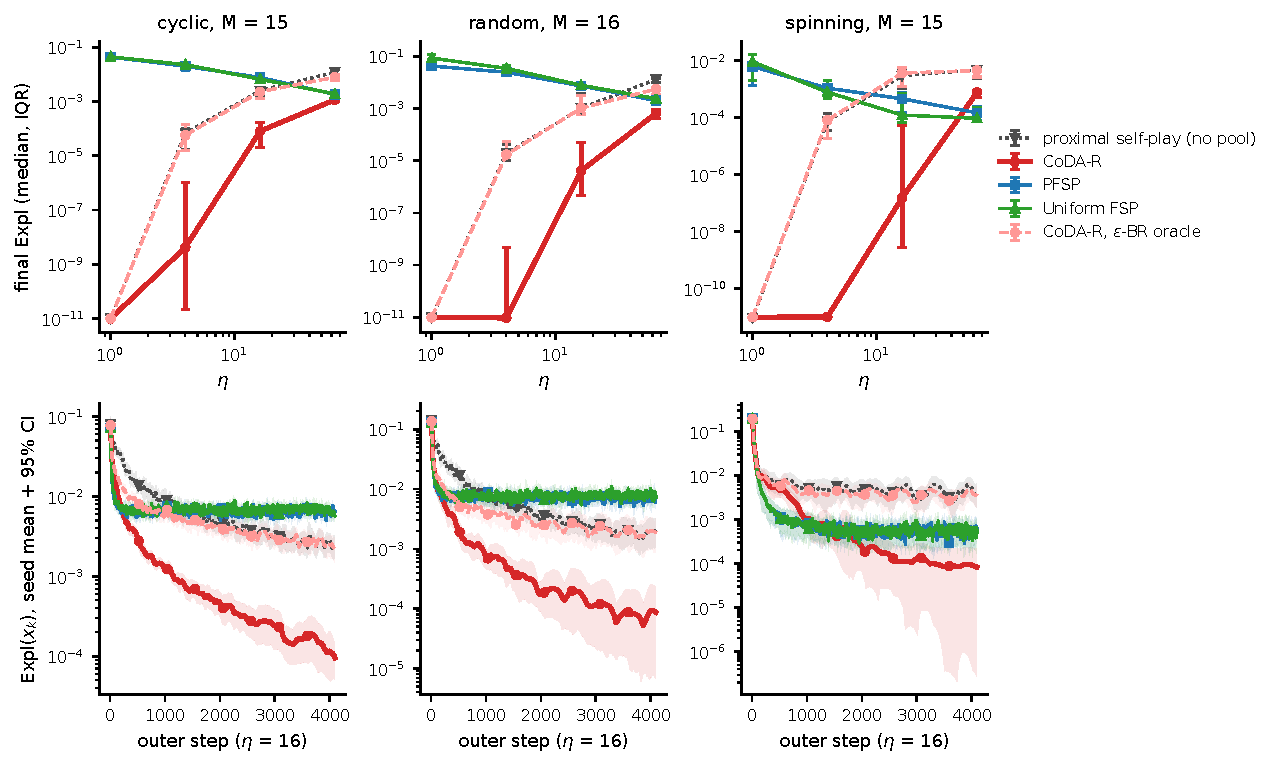
\includegraphics[width=0.92\linewidth]{figures/theory_oracle_rate.pdf}
\end{center}
\vspace{-6pt}
\caption{最佳响应 oracle 对精确算法的作用（每个博弈族 10 个博弈）。上：最终 exploitability 随 $\eta$ 的变化（中位数与四分位距）。下：$\eta=16$ 时 exploitability 随步数的变化。Proximal self-play 是空池的 \codar{}；PFSP 与 Uniform FSP 使用与 \codar{} 相同的池。}
\label{fig:oracle-rate}
\end{figure}

\textbf{oracle 的加速。}最佳响应 oracle 对 \codar{} 的加速符合定理~\ref{thm:oracle} 的预测（图~\ref{fig:oracle-rate}）。每一步都把策略锚的精确最佳响应加入池时，定理中的不等式在全部 240 次 \codar{} 运行的每一步都成立。对每个 $\eta\ge4$ 与全部三个博弈族，\codar{} 最终的 exploitability 都低于空池，例如 $\eta=16$ 时在随机 $16\times16$ 博弈上为 $4\times10^{-6}$ 对 $10^{-3}$；$\eta=1$ 时两者都到达数值下限。同一个池上的 PFSP 与均匀权重在 $\eta$ 较小时停在 $10^{-2}$ 附近，因为它们在均衡处仍把固定份额留给与学习者打平的 exploiter。误差为 $0.01$ 的 oracle 只在 exploitability 高于其误差的量级时有帮助，最终与空池接近，与定理的提示一致。这个排序有一处例外：在 spinning-top 博弈、$\eta=64$ 时，PFSP 与均匀权重的最终值更低（$1.5\times10^{-4}$ 与 $9.5\times10^{-5}$，对 $7.6\times10^{-4}$）。

\subsection{同预算对比}
\label{sec:exp-neural}

我们在 OpenSpiel\citep{lanctot2019openspiel} 的 Leduc 扑克\citep{southey2005bayesbluff}、Goofspiel(4)\citep{ross1971goofspiel} 与每人一颗骰子的 Liar's Dice\citep{lisy2015oos} 上，把 \codar{} 与七个基线比较。单网络基线有 PPO 自博弈；两个正则化自博弈方法 \rnad{} 与 MMD-PPO，分别用奖励塑形与 KL 损失实现近端项；以及两个池方法，均匀虚拟自博弈（Uniform FSP）与 PFSP。池方法与 \codar{} 共用对手池、oracle、败率估计器与策略更新，只在把败率估计映射为权重的规则上不同，所以 \codar{} 与 PFSP 的比较隔离出了权重规则的作用。混合基线有使用 PPO 最佳响应的 PSRO 与 Neural Fictitious Self-Play（NFSP）\citep{heinrich2016nfsp}。我们还运行了不带 oracle 的 \codar{}，以及作为上界对照的、使用不消耗对局的精确最佳响应（BR）oracle 的 \codar{}、PFSP 与 PSRO。所有 PPO 方法共用网络与 PPO 超参数，每个方法都在留出的 seed 上按同一套两阶段协议调参（附录~\ref{app:impl}）。每次运行的预算为 $B=4\times10^6$ 局，计入该方法消耗的全部对局，包括 exploiter 的训练与评估。我们报告全树精确 exploitability，Leduc 以筹码为单位，其余博弈以 $\pm1$ 的收益为单位，并用\emph{末段 exploitability}，即预算最后 20\% 上的平均，概括每次运行。表中给出 10 个 seed 上的四分位均值（IQM）与 bootstrap 95\% 置信区间（CI）\citep{agarwal2021precipice}，以及逐 seed 的配对差。

\begin{figure}[t]
\begin{center}
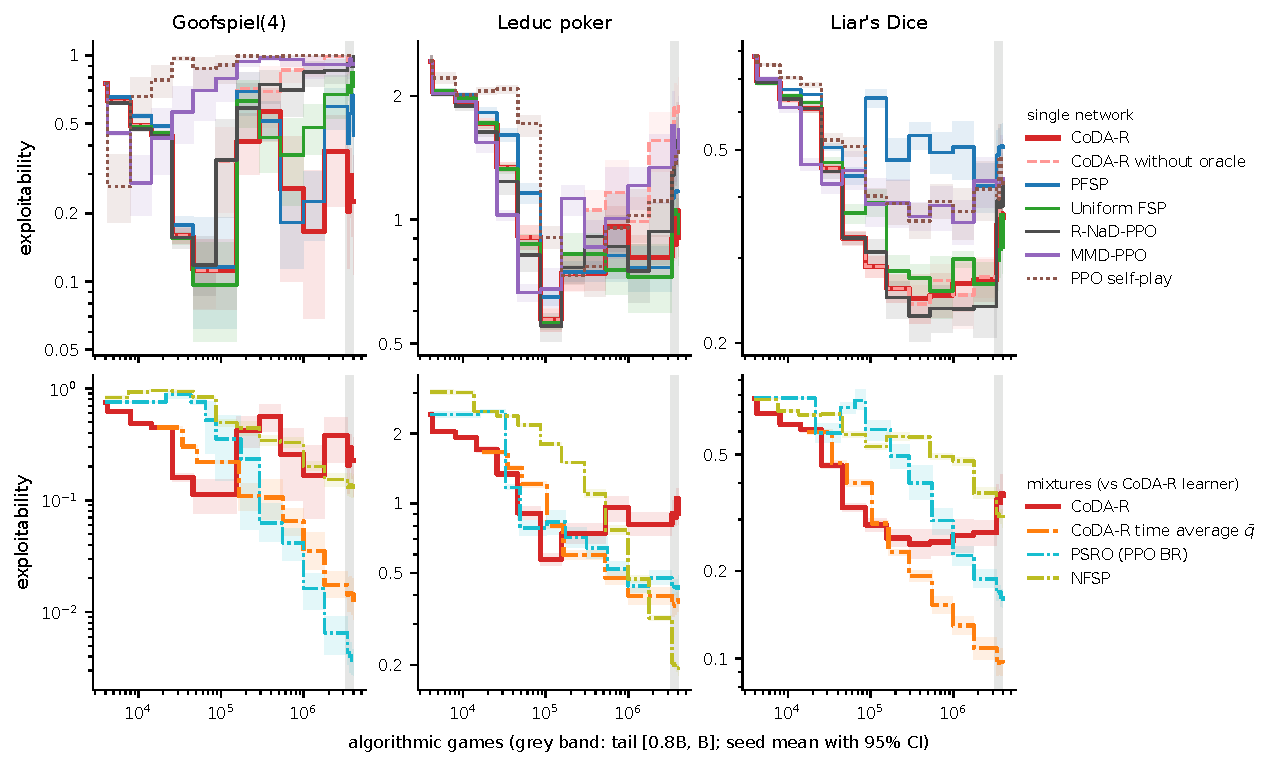
\includegraphics[width=0.95\linewidth]{figures/main_curves.pdf}
\end{center}
\vspace{-6pt}
\caption{训练过程中的精确 exploitability（10 个 seed 的均值与 95\% CI）。上：单网络。下：混合，并重复画出 \codar{} 的学习者作为参照。灰带为预算的最后 20\%。}
\label{fig:main}
\end{figure}

\begin{table}[t]
\caption{同预算下的末段 exploitability（10 个 seed 的 IQM [95\% CI]；越低越好）。粗体为每个博弈中最好的单网络。精确 BR 各行是上界对照。更多指标见附录表~\ref{tab:main-full}。}
\label{tab:main}
\begin{center}
\scriptsize
\setlength{\tabcolsep}{3pt}
\begin{tabular}{llccc}
\toprule
方法 & 部署 & Goofspiel(4) & Leduc 扑克 & Liar's Dice \\
\midrule
PPO 自博弈 & 单网络 & 0.999 [0.997, 1.000] & 1.287 [1.064, 1.705] & 0.445 [0.379, 0.501] \\
\rnad{} & 单网络 & 0.941 [0.858, 0.997] & 1.433 [1.345, 1.572] & 0.390 [0.360, 0.433] \\
MMD-PPO & 单网络 & 0.943 [0.863, 0.990] & 1.618 [1.416, 1.825] & 0.442 [0.368, 0.494] \\
Uniform FSP & 单网络 & 0.732 [0.662, 0.807] & 1.030 [0.928, 1.125] & \textbf{0.307} [0.286, 0.351] \\
PFSP & 单网络 & 0.517 [0.445, 0.590] & 1.150 [0.932, 1.297] & 0.479 [0.447, 0.502] \\
\codar{}（无 oracle） & 单网络 & 0.973 [0.866, 0.997] & 1.699 [1.483, 1.931] & 0.379 [0.316, 0.434] \\
\codar{} & 单网络 & \textbf{0.256} [0.221, 0.295] & \textbf{0.919} [0.880, 0.975] & 0.355 [0.322, 0.378] \\
\midrule
NFSP & 混合 & 0.116 [0.102, 0.164] & 0.196 [0.192, 0.200] & 0.308 [0.290, 0.329] \\
PSRO (PPO BR) & 混合 & 0.0040 [0.0031, 0.0050] & 0.433 [0.394, 0.480] & 0.163 [0.156, 0.172] \\
\codar{} 时间平均 $\bar{\bq}$ & 混合 & 0.0114 [0.0088, 0.0194] & 0.373 [0.324, 0.417] & 0.094 [0.084, 0.110] \\
\midrule
\codar{}，精确 BR oracle & 单网络 & 0.215 [0.138, 0.308] & 0.885 [0.797, 0.973] & 0.269 [0.241, 0.294] \\
PFSP，精确 BR oracle & 单网络 & 0.343 [0.301, 0.409] & 0.709 [0.625, 0.778] & 0.401 [0.375, 0.428] \\
PSRO，精确 BR & 混合 & $<10^{-15}$ & 0.108 [0.106, 0.115] & 0.172 [0.168, 0.175] \\
\bottomrule
\end{tabular}
\end{center}
\end{table}

\begin{table}[t]
\caption{末段 exploitability 的逐 seed 配对差（前者减后者；IQM [95\% CI]），括号内为 10 个 seed 中前者更好的个数。}
\label{tab:paired}
\begin{center}
\scriptsize
\setlength{\tabcolsep}{2.5pt}
\begin{tabular}{lccc}
\toprule
配对 & Goofspiel(4) & Leduc 扑克 & Liar's Dice \\
\midrule
\codar{} $-$ \rnad{} & $-0.659$ [$-0.747$, $-0.586$] (10) & $-0.503$ [$-0.662$, $-0.399$] (10) & $-0.051$ [$-0.097$, $-0.005$] (8) \\
\codar{} $-$ MMD-PPO & $-0.677$ [$-0.753$, $-0.554$] (10) & $-0.713$ [$-0.897$, $-0.519$] (10) & $-0.097$ [$-0.149$, $-0.034$] (9) \\
\codar{} $-$ PFSP & $-0.261$ [$-0.331$, $-0.163$] (10) & $-0.204$ [$-0.373$, $-0.017$] (7) & $-0.131$ [$-0.187$, $-0.065$] (10) \\
\codar{} $-$ Uniform FSP & $-0.500$ [$-0.580$, $-0.388$] (10) & $-0.139$ [$-0.218$, $+0.014$] (7) & $+0.045$ [$-0.033$, $+0.084$] (3) \\
\codar{} $-$ \codar{}（无 oracle） & $-0.693$ [$-0.769$, $-0.574$] (10) & $-0.761$ [$-1.010$, $-0.588$] (10) & $-0.037$ [$-0.077$, $+0.013$] (7) \\
\codar{} $-$ PFSP（均为精确 BR） & $-0.089$ [$-0.224$, $-0.020$] (10) & $+0.200$ [$+0.071$, $+0.293$] (2) & $-0.122$ [$-0.165$, $-0.095$] (10) \\
$\bar{\bq}$ $-$ PSRO (PPO BR) & $+0.007$ [$+0.004$, $+0.016$] (0) & $-0.078$ [$-0.112$, $-0.007$] (8) & $-0.069$ [$-0.089$, $-0.046$] (10) \\
$\bar{\bq}$ $-$ NFSP & $-0.106$ [$-0.146$, $-0.091$] (10) & $+0.178$ [$+0.128$, $+0.218$] (0) & $-0.208$ [$-0.220$, $-0.199$] (10) \\
\bottomrule
\end{tabular}
\end{center}
\end{table}

在单网络中，\codar{} 在 Goofspiel(4) 与 Leduc 扑克上的末段 exploitability 最低（表~\ref{tab:main} 与表~\ref{tab:paired}）。在这两个博弈上，它在全部 10 个 seed 上都优于 \rnad{}、MMD-PPO 与不带 oracle 的 \codar{}，末段 exploitability 比 \rnad{} 分别低 73\% 与 36\%。与只在权重规则上不同的 PFSP 相比，它在 Goofspiel(4) 上 10/10 个 seed 更好，在 Leduc 上 7/10 个 seed 更好。在 Liar's Dice 上，它优于 \rnad{}、MMD-PPO 与 PFSP，排在 Uniform FSP 之后，两者配对差的 CI 包含零。

不带池的方法在早期达到最低点之后退化，\codar{} 则基本保持住了水平（图~\ref{fig:main}）。在 Goofspiel(4) 与 Leduc 上，不带池的方法在预算的前 10\% 内达到各自最低的 exploitability，最终比最低点高 0.7--1.1，而 \codar{} 最终比自己的最低点高 0.25--0.36（附录表~\ref{tab:degradation}）。去掉 oracle 后，\codar{} 在这两个博弈上失去大部分增益，所以增益来自进入池的 exploiter。\codar{} 剩下的尖峰（在 Goofspiel(4) 上末段最差 exploitability 为 0.80）来自败率估计滞后于真实败率的突变：在那里检测到的 17 个漏洞中，有 14 个在出现时权重低于 0.01；在 \S\ref{sec:exp-abl} 的消融中，使用精确的成员败率降低了末段 exploitability。

更强的 oracle 在 Liar's Dice 上帮助了 \codar{}（$0.355\to0.269$），在另外两个博弈上变化不大。都使用精确最佳响应时，PFSP 在 Leduc 上领先（0.709 对 0.885）：那里 exploiter 的领先只占 26 筹码收益跨度的一小部分，所以权重 $c\mu/2$ 一直很小，而 PFSP 把固定的一半训练权重交给池。

同一次 \codar{} 运行的时间平均 $\bar{\bq}$ 与专门的混合方法相比有竞争力。它只需要每个外环步保存一个快照，在 Leduc（8/10 个 seed）与 Liar's Dice（10/10）上优于使用相同 PPO 最佳响应的 PSRO，在 Goofspiel(4) 上接近（0.011 对 0.004）；NFSP 在 Leduc 上更好。单个学习者在全部三个博弈上都高于这些混合。

exploiter 的领先给出校准良好的 exploitability 下界。oracle 的每次入池都给出 \S\ref{sec:oracle-rate} 中的下界 $[\ell(\hat\bx;\hat\by)-\tfrac12]^+$，由评估对局估计。在主实验的 3950 次入池中，单侧 95\% 置信下界超过真实 exploitability 3 次，为正（即提供了信息）2487 次。

\subsection{扩展到大型博弈}
\label{sec:exp-scale}

我们在 3$\times$3 abrupt Dark Hex 与 abrupt Phantom Tic-Tac-Toe 上训练六种方法。这是两个不完美信息博弈，约有 $2.7\times10^{10}$ 个节点，信息集分别为 $2.7\times10^{7}$ 与 $2.3\times10^{7}$ 个；预算相同，5 个 seed。各方法沿用在 Goofspiel(4) 上选出的配置，不再调参。exploitability 用 exp-a-spiel\citep{rudolph2025reevaluating} 在全树上精确计算，末段 exploitability 取 $0.8B$、$0.9B$ 与 $B$ 处三个 checkpoint 的平均。

\begin{table}[t]
\caption{大型博弈：末段 exploitability（5 个 seed 的 IQM [95\% CI]），以及逐 seed 配对差 \codar{} $-$ 方法，括号内为 5 个 seed 中 \codar{} 更好的个数。}
\label{tab:scale}
\begin{center}
\scriptsize
\setlength{\tabcolsep}{3pt}
\begin{tabular}{llcccc}
\toprule
 & & \multicolumn{2}{c}{3$\times$3 abrupt Dark Hex} & \multicolumn{2}{c}{Abrupt Phantom TTT} \\
方法 & 部署 & 末段 exploitability & \codar{} $-$ 方法 & 末段 exploitability & \codar{} $-$ 方法 \\
\midrule
PPO 自博弈 & 单网络 & 0.971 [0.837, 0.993] & $-0.531$ [$-0.592$, $-0.376$] (5) & 0.961 [0.893, 0.985] & $-0.439$ [$-0.464$, $-0.409$] (5) \\
\rnad{} & 单网络 & 0.529 [0.438, 0.598] & $-0.108$ [$-0.174$, $+0.023$] (4) & \textbf{0.509} [0.490, 0.568] & $-0.009$ [$-0.062$, $+0.041$] (2) \\
MMD-PPO & 单网络 & 0.542 [0.524, 0.583] & $-0.109$ [$-0.182$, $-0.054$] (5) & 0.641 [0.604, 0.751] & $-0.126$ [$-0.279$, $-0.062$] (5) \\
PFSP & 单网络 & 0.743 [0.710, 0.794] & $-0.333$ [$-0.361$, $-0.237$] (5) & 0.832 [0.773, 0.893] & $-0.316$ [$-0.402$, $-0.246$] (5) \\
\codar{} & 单网络 & \textbf{0.432} [0.395, 0.476] & --- & 0.512 [0.467, 0.551] & --- \\
\midrule
PSRO (PPO BR) & 混合 & 0.355 [0.290, 0.386] & $+0.092$ [$+0.010$, $+0.159$] (0) & 0.525 [0.495, 0.529] & $-0.014$ [$-0.061$, $+0.055$] (4) \\
\bottomrule
\end{tabular}
\end{center}
\end{table}

\codar{} 在 Dark Hex 上的末段 exploitability 是单网络中最低的，在 Phantom Tic-Tac-Toe 上与 \rnad{} 持平，两者相差 0.009，CI 包含零（表~\ref{tab:scale}）。它在 Phantom Tic-Tac-Toe 上与 PSRO 的混合相当，在 Dark Hex 上落后 0.09。使用相同的池与 oracle 的 PFSP 在两个博弈上都差得多（0.74 与 0.83），自博弈则几乎完全可被利用。在最终策略之间的抽样循环赛中，\codar{} 在 Dark Hex 上的平均得分最高（0.510），在 Phantom Tic-Tac-Toe 上与最高分相差不到 0.001。让每个 checkpoint 与自己更早的 checkpoint 对局可以看到，只有自博弈会输给过去的自己，占其 checkpoint 的 25--29\%；对 \codar{}，更早的 checkpoint 的最大领先（在各 checkpoint 上平均）在 Dark Hex 上为 0.009，在 Phantom Tic-Tac-Toe 上为负（附录图~\ref{fig:scale-history}）。

\subsection{对手池带来什么}
\label{sec:exp-mech}

主实验中混着几种效应。我们在 Leduc 与 Goofspiel(4) 上做了四个受控实验把它们分开，每个实验 6 个 seed，沿用主实验的配置（设置与完整的表见附录~\ref{app:mech}）。

\begin{figure}[t]
\begin{center}
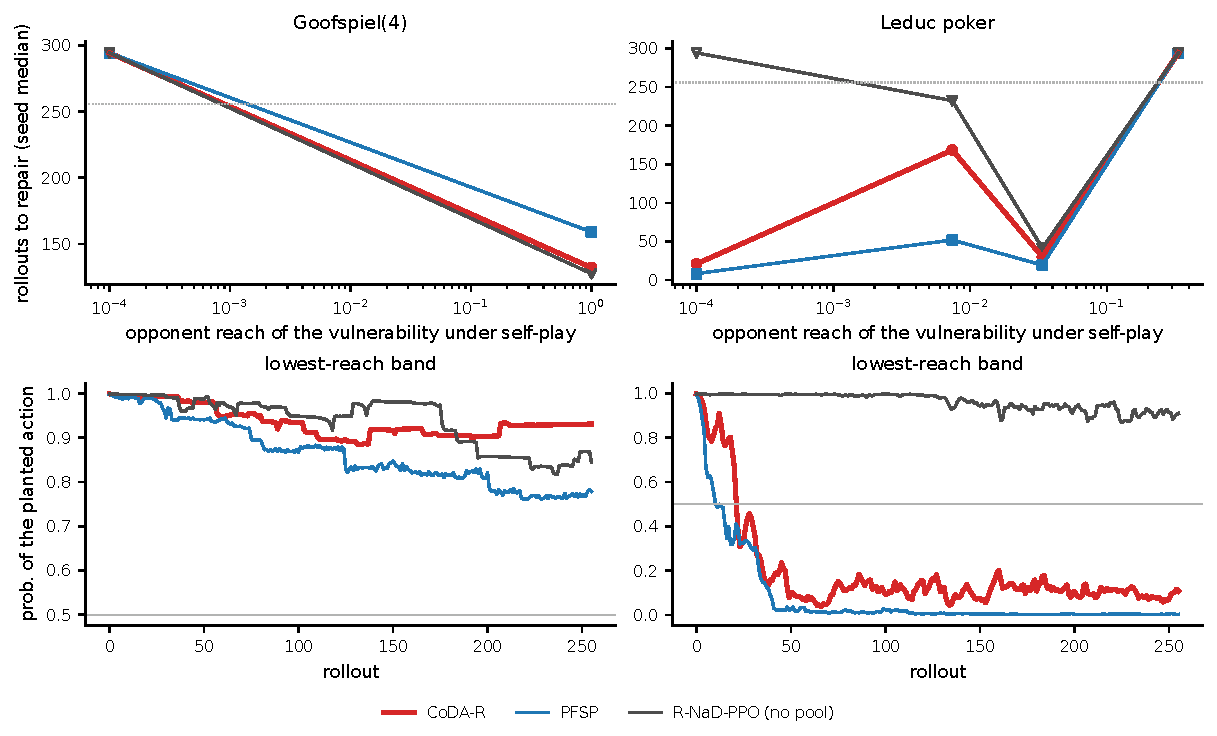
\includegraphics[width=0.78\linewidth]{figures/hidden_hole.pdf}
\end{center}
\vspace{-6pt}
\caption{隐藏漏洞（6 个 seed）。上：修复所需 rollout 数的中位数，横轴为自博弈对手到达所埋漏洞的概率；虚线以上的点表示未修复。下：对手到达概率最低一档中，所埋动作的概率。}
\label{fig:mech}
\end{figure}

\begin{figure}[t]
\begin{center}
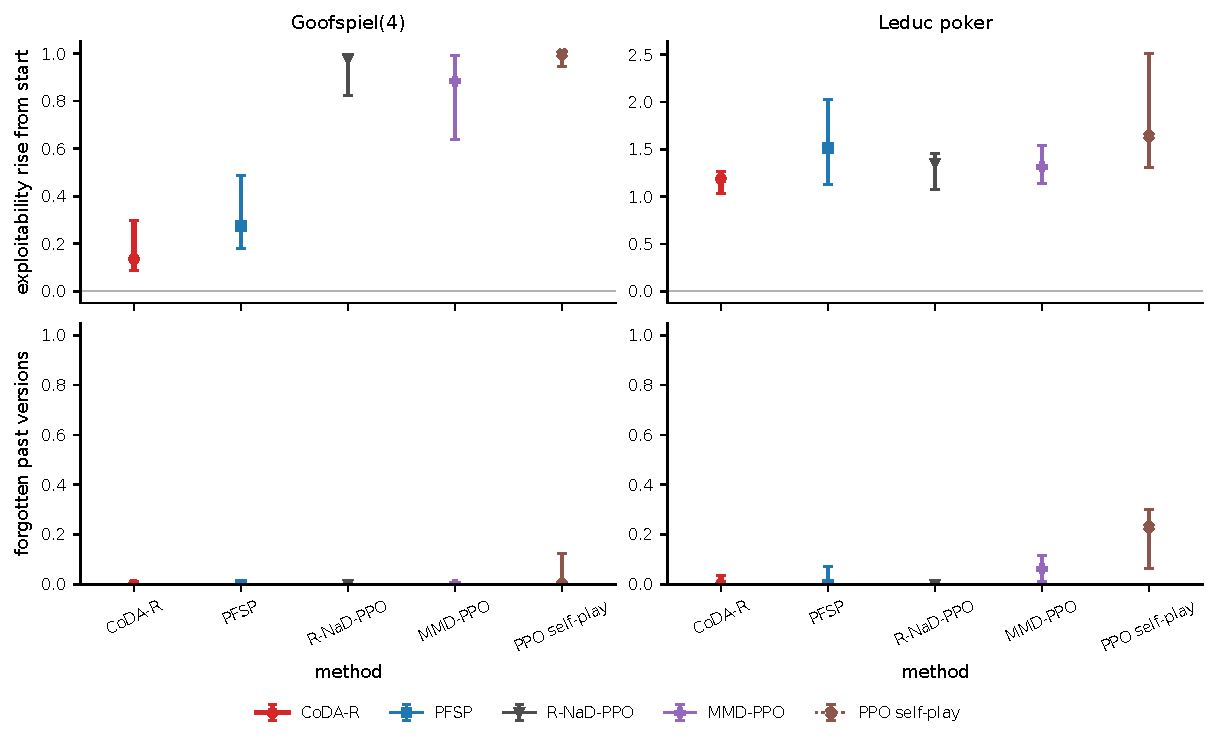
\includegraphics[width=0.78\linewidth]{figures/forgetting.pdf}
\end{center}
\vspace{-6pt}
\caption{从接近纳什的起点出发的保持情况（6 个 seed 的 IQM 与 95\% CI）。上：exploitability 相对起始网络的上升。下：归档的早先版本中，后来又击败学习者的比例。}
\label{fig:retention}
\end{figure}

\textbf{隐藏漏洞。}对手池能修补自博弈几乎走不到的漏洞。我们把 counterfactual regret minimization（CFR+）\citep{tammelin2014cfrplus}的平均策略蒸馏进一个网络，并在这样的信息集上埋入漏洞：学习者自己经常到达，而自博弈对手以受控的概率到达，概率从 $[0.3,1)$ 一直到 $10^{-3}$ 以下。池里只有受损网络的精确最佳响应，\rnad{} 的训练不使用它。在 Leduc 上（图~\ref{fig:mech}），\rnad{} 的修复时间随对手到达概率的降低而变长；在到达概率约 $2\times10^{-6}$ 的最低一档，它在 256 个 rollout 内 6 个 seed 一个也没有修复。攻击者在池里时，\codar{} 在全部 6 个 seed 上修复了漏洞（中位数 21 个 rollout），PFSP 也是如此（中位数 8.5）。PFSP 更快，是因为它给攻击者约 0.17 的固定系数，而 \codar{} 给的是 0.03--0.06，它的权重跟随攻击者约 0.02 的小幅领先。固定系数的代价是 exploitability：在最低一档，PFSP 最终为 1.61，\codar{} 为 1.30，\rnad{} 为 1.81。在 Goofspiel(4) 上，没有方法修复最低一档，因为学习者在别的分支上反制了这个确定性的攻击者，攻击者不再赢，而漏洞依然存在。

\textbf{保持。}对手池能让接近纳什的网络留在纳什附近。从同一个蒸馏网络出发，不埋漏洞（exploitability 在 Goofspiel(4) 上为 $3.8\times10^{-4}$，在 Leduc 上为 $0.0088$），每种方法再训练 $10^6$ 局。在 Goofspiel(4) 上（图~\ref{fig:retention}），不带池的方法几乎完全丢掉了均衡：exploitability 的上升，\rnad{} 为 0.98，MMD-PPO 为 0.88，自博弈为 1.00。\codar{} 上升 0.14 [0.09, 0.30]，在全部 6 个 seed 上都小于每个不带池的方法；PFSP 上升 0.28，所以保持是对手池带来的性质。在 Leduc 上，每种方法都漂回主实验中各自的水平附近，其中 \codar{} 上升得最少（1.19 对 1.32--1.64；只对自博弈显著）。漂移集中在自博弈走不到的地方。在自博弈对手到达概率低于 $10^{-3}$ 的信息集上，Leduc 上相对起点的每次到达损失，\codar{} 为 0.0030，PFSP 为 0.0040，不带池的方法为 0.0093--0.0157，而到达概率较高的各档差别不大（附录图~\ref{fig:drift}）。可见隐藏漏洞与漂移出自同一个机制：自博弈在它走不到的地方不产生梯度，参数共享使策略的这些部分发生漂移，而会走到那里的池成员补上了缺失的信号。循环回到已被击败的版本则是另一种效应，单靠近端项就能避免：面对自己早先版本的归档，只有自博弈（Leduc 上 23\% 的版本）与 MMD-PPO（6\%）会输给曾经击败过的版本。把 $c$ 减半或加倍不改变这些结果。

\textbf{沉睡成员。}成员一旦重新开始赢，\codar{} 就立刻把权重还给它，并且很少把训练花在不再赢的成员上。累计历史的权重（如 Hedge）会让一个被压制了 $T$ 轮的成员“沉睡”：它必须再赢大约 $T$ 轮才能拿回权重。我们把一个 \rnad{} 底座网络的精确最佳响应与三个随机网络诱饵一起放进池，让每种规则把它压制 $T\in\{24,48,96,192\}$ 个 rollout，然后把学习者重置回底座，重新打开这个漏洞。对 \codar{}，再次修复所需的时间与 $T$ 无关（Goofspiel(4) 上约 1 个 rollout，Leduc 上 3--6 个）。Hedge 在 $T=192$ 时需要 31.5 与 37.7 个 rollout（附录图~\ref{fig:sleeper}），不带池的 \rnad{} 在 Leduc、$T=192$ 时 96 个 rollout 内没有再次修复。不能击败学习者的成员（$\ell\le0.51$）在 \codar{} 下，在 Goofspiel(4) 上持有 0.6--1.5\% 的训练权重，在 Leduc 上持有 11--13\%，而 PFSP 与 Hedge 为 44--50\%，固定比例为 28--35\%。在 Leduc 上，这一设置下固定份额的规则最终的末段 exploitability 更低（PFSP 为 0.57--0.65，固定比例为 0.48--0.59，对 0.72--0.81）。移动锚在这里的表现与 \codar{} 相同，因为它的失败需要一个打平的池。

\textbf{开放池。}池由外部智能体组成且没有 oracle 时，\codar{} 把训练留给仍能击败学习者的成员。外部成员为 4 到 64 个（早期的 CFR+ 迭代、小的旧版网络、脚本对手、均匀策略、随机网络及重复成员）时，学习者已经击败的成员在 \codar{} 下，在 Goofspiel(4) 上持有 0.3--1.1\% 的训练权重，在 Leduc 上持有 4--6\%，而在 PFSP 下为 42--46\%，在 Uniform FSP 下为 9--19\%，且与池的大小无关（附录图~\ref{fig:open-pool}）。此时每种规则下的 exploitability 都取决于池成员知道什么，而这个池在没有 oracle 时不能稳定地降低它。

\subsection{消融}
\label{sec:exp-abl}

附录图~\ref{fig:ablations} 每次只改变 \codar{} 的一个设计要素（$10^6$ 局，6 个 seed，与基准配置配对）。oracle 最重要：去掉它使末段 exploitability 在 Goofspiel(4) 上升高 0.76，在 Leduc 上升高 0.42。在整个外环步内冻结池权重会破坏 \S\ref{sec:primal} 的隐式配对，代价为 0.38 与 0.15；池容量取 4 的代价为 0.32 与 0.24。精确的成员败率（$\xi_k=0$）在 Goofspiel(4) 上有帮助（$-0.09$，6/6 个 seed），说明估计滞后是那里剩下的主要误差；把 oracle 占预算的份额加倍到 24\% 在 Leduc 上有帮助（$-0.20$，5/6 个 seed）。移动对偶锚、采样分布、自博弈对手的刷新频率，以及 KL 形式的近端项，在这个预算下对末段 exploitability 的影响都在 CI 之内；移动锚的失败出现在 \S\ref{sec:exp-theory} 的精确设置中。

% ----------------------------------------------------------------------
\section{相关工作}
\label{sec:related}
% ----------------------------------------------------------------------

对手池方法保留一池对手，把均衡放在混合里。Double Oracle 与 PSRO\citep{mcmahan2003doubleoracle,lanctot2017psro,muller2020generalized,mcaleer2020pipeline}在外部求解池上的元博弈\citep{wellman2006egta}，PFSP 与联赛训练\citep{vinyals2019alphastar}按胜率分配采样比例，NFSP\citep{heinrich2015fsp,heinrich2016nfsp}用一个单独的网络学习历史平均策略。它们部署的是 checkpoint 的混合或平均网络。\codar{} 使用同样的池与 oracle，并把保证留在正在训练的网络上。

正则化自博弈给出单个网络的保证，但没有对手池。R-NaD 与 MMD\citep{perolat2021rnad,perolat2022stratego,sokota2023mmd}在收益或策略空间使用一个周期移动或逐渐退火的锚，乐观与外梯度方法\citep{daskalakis2018optimism,mertikopoulos2019omd,nemirovski2004prox,cen2021extragradient}用外推项起到类似的稳定作用；两者都是近端点法\citep{rockafellar1976ppa}的显式近似\citep{mokhtari2020ppa}。它们只沿自博弈的轨迹训练，这也是 OpenAI Five 与 AlphaStar 额外保留历史对手的原因\citep{openai2019dota,vinyals2019alphastar,czarnecki2020spinning}。\codar{} 的策略更新就是近端点法的一步，池为空时 \codar{} 退化为近端点法。

乘性权重会累计历史，\codar{} 的无状态投影避免了这一点。PSRO 一族的元求解器，即 Hedge、投影复制子动力学与乘性权重更新（MWU），以及 OpenAI Five 的对手采样器，多数使用乘性权重\citep{lanctot2017psro,mcaleer2022anytime,dinh2022odo,openai2019dota,freund1999hedge}。一个成员被压制 $T$ 轮之后，即使重新克制学习者，也要再赢大约 $T$ 轮才能拿回权重。这就是在线学习中 Fixed Share 类算法所处理的沉睡问题\citep{herbster1998tracking}。反过来，打平的成员会一直保留正的权重。部署时间平均的方法不受影响，但乘性权重的 last-iterate 在零和博弈中不收敛\citep{bailey2018mwu}，保留着权重的打平成员还可能把学习者钉在非纳什点上（命题~\ref{prop:rps}）。附录表~\ref{tab:related} 给出各方法的对照。

% ----------------------------------------------------------------------
\section{结论}
% ----------------------------------------------------------------------

\codar{} 让单个网络与自己、与开放的对手池对局。把对偶锚固定在纯自博弈上，把移动锚放在策略更新里，就使策略移动与池权重共用一笔预算，即到均衡的距离。对精确算法，由此得到所训练的策略对任意池序列的 last-iterate 收敛、显式的速率，以及最佳响应 oracle 的定量增益。在 PPO 实现上，以相同的预算、与按同一协议调参的基线相比，\codar{} 的学习者在 Goofspiel(4)、Leduc 扑克与 3$\times$3 abrupt Dark Hex 上取得单网络中最低的末段 exploitability，在 abrupt Phantom Tic-Tac-Toe 上与 \rnad{} 持平，在 Liar's Dice 上排在 Uniform FSP 之后。受控实验表明，对手池能修补自博弈几乎走不到的漏洞，并让接近纳什的网络留在原地；权重规则会把权重立刻还给重新打开的漏洞，并且很少把训练花在不再赢的成员上。由于权重跟随对手的领先幅度，小幅的领先修复得比 PFSP 的固定份额慢。更快地发现小幅领先、欧氏理论的 KL 版本，以及跨越池变化的 last-iterate 速率，是主要的开放方向。

\subsubsection*{可复现性声明}
\S\ref{sec:prelim}--\ref{sec:alg} 给出算法的全部定义，\S\ref{sec:theory} 与附录~\ref{app:proofs} 给出全部证明。\S\ref{sec:impl} 与附录~\ref{app:impl} 给出实现、评估协议、调参网格与每个选定的配置。源代码包括有限维求解器与检查、PPO 实现、全部基线、带有全部配置与 seed 的实验入口，以及从原始输出生成每一张图与表的脚本；代码开源在作者的 GitHub：\url{https://github.com/GICF-E/CoDA-R}。

\subsubsection*{AI 使用声明}
在本工作中，我们使用生成式 AI 工具协助起草与润色论文文字、编写与重构实验代码、整理参考文献格式，以及汇总实验日志以生成图表。在研究内容方面，AI 工具被用于打磨研究假设的表述、协助推导与检查证明步骤，以及协助解读实验结果。核心算法、定理陈述与研究设计由作者提出。我们没有使用生成式 AI 生成合成数据或伪造实验结果。所有 AI 协助的代码都经过作者的测试与类型检查，所有 AI 协助的证明、解读与文字都经过作者逐项人工审阅。作者对本文的全部内容负责。

\bibliography{references}
\bibliographystyle{plainnat}

% ----------------------------------------------------------------------
\appendix
\section{证明}
\label{app:proofs}
% ----------------------------------------------------------------------

正文证明了引理~\ref{lem:A}、引理~\ref{lem:B} 与定理~\ref{thm:energy}。本附录按出现的顺序证明其余结论，只用到 \S\ref{sec:prelim} 列出的工具。全文简记 $\bx:=\bx_{k+1}$、$\bw:=\bw(\bx)$、$\bv:=\bv_{k+1}$、$\dx_k=\bx_{k+1}-\bx_k$。

\subsection{引理~\ref{lem:dual}：权重规则的性质}
\label{app:dual}

记 $\bz:=\esp+c\aug(\bx)$，于是 $\bw=\Proj_\simplex(\bz)$；记 $z_{\mathrm{sp}}=1+\tfrac c2$ 为 $\bz$ 的自博弈坐标。

(a) 由投影不等式，$\esp=\Proj_\simplex(\bz)$ 当且仅当对所有 $\bu\in\simplex$ 有 $(\bz-\esp)^\top(\bu-\esp)\le0$。由于 $\bz-\esp=c\aug$，这个条件变为对所有 $\bu$ 有 $\aug^\top \bu\le\aug^\top \esp=\tfrac12$。线性函数在单纯形上的最大值在顶点取到，所以这等价于 $\max_j\tilde\ell_j\le\tfrac12$。自博弈坐标恰为 $\tfrac12$，故又等价于 $\max_{i\in P}\ell_i\le\tfrac12$。

(b) 把一点权重从成员 $i$ 挪给自博弈：取 $\bu=\bw+\theta(\esp-\be_i)$，$0<\theta\le w_i$，它仍在 $\simplex$ 中。由投影不等式，
\[
(\bz-\bw)^\top(\bu-\bw)=\theta\big[(z_{\mathrm{sp}}-\wsp)-(z_i-w_i)\big]\le0
\iff c\,\ell_i-w_i\ \ge\ z_{\mathrm{sp}}-\wsp=1+\tfrac c2-\wsp ,
\]
即 $c(\ell_i-\tfrac12)\ge1-\wsp+w_i\ge w_i>0$。

(c) $\simplex_2$ 中的点为 $(\theta,1-\theta)$，$\theta\in[0,1]$，它到 $\bz=(\tfrac c2+c\mu,\ 1+\tfrac c2)$ 的距离平方
\[
(\tfrac c2+c\mu-\theta)^2+(\tfrac c2+\theta)^2
\]
是 $\theta$ 的凸二次函数，无约束最小点为 $\theta=\tfrac{c\mu}2$；在 $[0,1]$ 上的最小点就是把它截断到这个区间。\hfill$\blacksquare$

\subsection{策略更新的解唯一}
\label{app:unique}

\begin{proposition}[每一步的解唯一]
\label{prop:unique}
对任意策略锚 $\bx_k$ 与任意池，\eqref{eq:P} 有且只有一个解。
\end{proposition}
唯一性来自三个事实：自博弈项是反对称的，池项由投影的单调性是单调的，近端项是 $\eta$-强单调的。存在性由 Hartman--Stampacchia 定理得到。记前两项的算子为 $G_k(\bx):=S\bx+A\bw(\bx)_P$。

\textit{$G_k$ 单调。}对自博弈项，$(\bx-\bx')^\top S(\bx-\bx')=0$，故 $\langle S(\bx-\bx'),\bx-\bx'\rangle=0$。对池项，记 $\bz=\esp+c\aug(\bx)$、$\bz'=\esp+c\aug(\bx')$。两者的自博弈坐标相同，池坐标相差 $c(\ell_i(\bx)-\ell_i(\bx'))=c\,(S\by_i)^\top(\bx-\bx')$，即 $(\bz-\bz')_P=c\,A^\top(\bx-\bx')$。由 \eqref{eq:monotone}，
\[
0\le(\bz-\bz')^\top\big(\bw(\bx)-\bw(\bx')\big)=(\bz-\bz')_P^\top\big(\bw(\bx)-\bw(\bx')\big)_P=c\,(\bx-\bx')^\top A\big(\bw(\bx)-\bw(\bx')\big)_P ,
\]
即 $\langle A\bw(\bx)_P-A\bw(\bx')_P,\bx-\bx'\rangle\ge0$。加上 $\eta(\bx-\bx_k)$ 之后，整个算子满足 $\langle\cdot,\bx-\bx'\rangle\ge\eta\|\bx-\bx'\|^2$，即它是 $\eta$-强单调的。这里用到自博弈系数与 $\bx$ 无关；若系数取 $\wsp(\bx)$，自博弈项成为 $\wsp(\bx)S\bx$，不再是反对称的二次型。

\textit{唯一性。}设 $\bx$ 与 $\bx'$ 都是 \eqref{eq:P} 的解。在 $\bx$ 的不等式中取测试点 $\bx'$，在 $\bx'$ 的不等式中取测试点 $\bx$：
\[
\langle G_k(\bx)+\eta(\bx-\bx_k),\,\bx'-\bx\rangle\ge0,\qquad\langle G_k(\bx')+\eta(\bx'-\bx_k),\,\bx-\bx'\rangle\ge0 .
\]
两式相加得 $\eta\|\bx-\bx'\|^2\le-\langle G_k(\bx)-G_k(\bx'),\bx-\bx'\rangle\le0$，故 $\bx=\bx'$。

\textit{存在性。}$\aug$ 是仿射的，$\bw(\bx)$ 由 \eqref{eq:monotone} 的非扩张性是连续的，所以 $G_k$ 连续，而 $X$ 是紧凸集。紧凸集上连续算子的变分不等式有解，这就是 Hartman--Stampacchia 定理\citep{hartman1966,facchinei2003vi}。\hfill$\blacksquare$

\subsection{定理~\ref{thm:cert}：两条证书}
\label{app:cert}

(i) 取 $\by_e\in\arg\max_\by\ell(\bx;\by)$。则 $\bx^\top S\by_e=\Expl(\bx)$，由反对称性 $\by_e^\top S\bx=-\Expl(\bx)$。在 \eqref{eq:P} 中取 $\bx'=\by_e$，记 $\bg:=\by_e-\bx$，把三项分开：
\[
\underbrace{(S\bx)^\top \bg}_{\text{自博弈}}+\underbrace{(A\bw_P)^\top \bg}_{\text{池}}+\underbrace{\eta\,\dx_k^\top \bg}_{\text{近端}}\ \ge\ 0 .
\]
自博弈项为 $(S\bx)^\top \bg=\by_e^\top S\bx-\bx^\top S\bx=-\Expl(\bx)$。对池项，利用 $(S\by_i)^\top \bz=\ell_i(\bz)-\tfrac12$，
\[
(A\bw_P)^\top \bg=\sum_iw_i\big(\ell_i(\by_e)-\ell_i(\bx)\big)=\sum_iw_i\big(\ell_i(\by_e)-\tfrac12\big)-b\ \le\ \tfrac12a-b ,
\]
最后一步用到败率不超过 1。对近端项，由 Cauchy--Schwarz 与直径，$\eta\,\dx_k^\top \bg\le\eta D\|\dx_k\|$。三项合起来得 $-\Expl(\bx)+\tfrac12a-b+\eta D\|\dx_k\|\ge0$，整理即得第一个不等式；第二个不等式用到 $b\ge0$。

(ii) 对 $\bw=\Proj_\simplex(\esp+c\aug)$ 用投影不等式，取 $\bu=\be_j$，$j$ 为任一池成员：
\[
\big(\esp+c\aug-\bw\big)^\top(\be_j-\bw)\le0\iff c\,\aug^\top(\be_j-\bw)\le(\bw-\esp)^\top(\be_j-\bw)\le\sqrt2\,\|\bw-\esp\| .
\]
由 \eqref{eq:identities}，左端等于 $c(\ell_j-\tfrac12-b)$，故 $\ell_j-\tfrac12\le\frac{\sqrt2}c\|\bw-\esp\|+b$。由引理~\ref{lem:B} 与 Cauchy--Schwarz，$b\le\eta\,\dx_k^\top(\xs-\bx)\le\eta D\|\dx_k\|$。取 $j$ 为败率最大的成员，右端非负，所以取正部不影响这个界。\hfill$\blacksquare$

\subsection{定理~\ref{thm:conv}：学习者的收敛}
\label{app:conv}

推论~\ref{cor:sum} 给出 $a\to0$ 与 $\|\dx_k\|\to0$，代入定理~\ref{thm:cert}(i) 得 $\Expl(\bx_{k+1})\le\tfrac12a+\eta D\|\dx_k\|\to0$。由于 $X$ 是紧的、$\Expl$ 连续，任一收敛子列的极限 $\bar \bx$ 都是纳什策略。定理~\ref{thm:energy} 对 $\xs=\bar \bx$ 成立，所以 $\|\bx_k-\bar \bx\|$ 不增；它沿子列趋于零，故沿整个序列趋于零。\hfill$\blacksquare$

\subsection{定理~\ref{thm:rate}：速率}
\label{app:rate}

\textit{(i) 的证明。}记 $\alpha_k=\|\bw(\bx_{k+1})-\esp\|$，$\beta_k=\|\dx_k\|$。由定理~\ref{thm:cert}(i) 与 $a\le\alpha_k$，$\Expl(\bx_{k+1})\le\tfrac12\alpha_k+\eta D\beta_k$。最小值不超过平均值；对两个和分别用 Cauchy--Schwarz（$\sum_{k<K}\alpha_k\le\sqrt K\sqrt{\sum\alpha_k^2}$），再代入推论~\ref{cor:sum}，
\begin{align*}
\min_{k<K}\Expl(\bx_{k+1})\ &\le\ \frac1K\sum_{k<K}\Big(\tfrac12\alpha_k+\eta D\beta_k\Big)\\
&\le\ \frac{1}{\sqrt K}\Big(\tfrac12\sqrt{\tfrac{c\eta}{2}}+\eta D\Big)\|\bx_0-\xs\|\ \le\ \frac{\sqrt{c\eta}/2+2\eta}{\sqrt K},
\end{align*}
最后一步用到 $\|\bx_0-\xs\|\le\sqrt2$ 与 $D=\sqrt2$。

\textit{池固定时移动量不增。}池固定时，相邻两步共用同一个算子 $G(\bx):=S\bx+A\bw(\bx)_P$，它是单调的（附录~\ref{app:unique}）。在第 $k$ 步的 \eqref{eq:P} 中取测试点 $\bx_{k+2}$，在第 $k+1$ 步中取 $\bx_{k+1}$：
\[
\langle G(\bx_{k+1})+\eta\dx_k,\ \bx_{k+2}-\bx_{k+1}\rangle\ge0,\qquad\langle G(\bx_{k+2})+\eta\dx_{k+1},\ \bx_{k+1}-\bx_{k+2}\rangle\ge0 .
\]
两式相加，$G$ 的部分由单调性 $\le0$，剩下 $\eta\langle\dx_k-\dx_{k+1},\dx_{k+1}\rangle\ge0$，即 $\|\dx_{k+1}\|^2\le\dx_k^\top\dx_{k+1}\le\|\dx_k\|\|\dx_{k+1}\|$，故 $\|\dx_{k+1}\|\le\|\dx_k\|$。

\textit{(ii) 的证明。}池在第 $K-n,\dots,K-1$ 步内不变，所以 $\|\dx_k\|$ 在这些步上不增。从 $\bx_{K-n}$ 起对能量不等式 \eqref{eq:energy} 求和，得 $n\|\dx_{K-1}\|^2\le\sum_{k=K-n}^{K-1}\|\dx_k\|^2\le\|\bx_{K-n}-\xs\|^2\le2$，即 $\beta:=\|\dx_{K-1}\|\le\sqrt{2/n}$。在 $\bx=\bx_K$ 处，引理~\ref{lem:B} 与 Cauchy--Schwarz 给出 $b(\bx)\le\eta D\beta$，引理~\ref{lem:A} 与 $a^2\le\|\bw-\esp\|^2$ 给出 $a(\bx)\le\sqrt{c\,b(\bx)}\le\sqrt{c\eta D\beta}$。代入定理~\ref{thm:cert}(i)，
\[
\Expl(\bx_K)\ \le\ \tfrac12\sqrt{c\eta D\beta}+\eta D\beta\ \le\ \sqrt{c\eta/2}\;n^{-1/4}+2\eta\,n^{-1/2},
\]
这里用到 $D=\sqrt2$。\hfill$\blacksquare$

\subsection{命题~\ref{prop:mix}：混合策略}
\label{app:mix}

\textit{(i) 的证明。}$\bq_{k+1}=\bv_{k+1}/t_k\in X$，因为 $\bv$ 是 $X$ 中若干点的非负组合，总质量为 $t_k\ge1$。对任意 $\by\in X$，在 \eqref{eq:P} 中取 $\bx'=\by$：
\[
\by^\top S\bv-\underbrace{\bx^\top S\bv}_{=b}+\eta\,\dx_k^\top(\by-\bx)\ge0
\ \Longrightarrow\
-\by^\top S\bv\ \le\ -b+\eta\,\dx_k^\top(\by-\bx)\ \le\ \eta D\|\dx_k\| .
\]
由反对称性，左端等于 $\bv^\top S\by=t_k\,\bq_{k+1}^\top S\by$，对 $\by$ 取最大值得 $t_k\Expl(\bq_{k+1})\le\eta D\|\dx_k\|$。

\textit{(ii) 的证明。}上面的中间一步 $-\by^\top S\bv_{k+1}\le\eta\,\dx_k^\top(\by-\bx_{k+1})$ 在每一步都成立。以 $\by$ 为参考点用极化恒等式，
\[
2\,\dx_k^\top(\by-\bx_{k+1})=\|\bx_k-\by\|^2-\|\bx_{k+1}-\by\|^2-\|\dx_k\|^2\ \le\ \|\bx_k-\by\|^2-\|\bx_{k+1}-\by\|^2 ,
\]
在 $k<K$ 上求和，
\[
T_K\,\bar{\bq}_K^\top S\by=-\by^\top S\sum_{k<K}\bv_{k+1}\ \le\ \tfrac\eta2\big(\|\bx_0-\by\|^2-\|\bx_K-\by\|^2\big)\ \le\ \tfrac\eta2\|\bx_0-\by\|^2\ \le\ \eta .
\]
两边除以 $T_K$ 并对 $\by$ 取最大值；$T_K\ge K$ 是因为每个 $t_k=1+a(\bx_{k+1})\ge1$。\hfill$\blacksquare$

\subsection{定理~\ref{thm:inexact}：非精确步}
\label{app:inexact}

记 $\hat b:=\sum_iw_{k+1,i}(\hat\ell_{k,i}-\tfrac12)$ 为由估计败率算出的池压力，$a$ 与 $b$ 则由实际权重与真实败率定义。

\textit{能量不等式。}引理~\ref{lem:A} 对实际被投影的向量成立，证明相同，只是把 $\aug$ 换成 $\hat{\bell}$，由此 $\|\bw_{k+1}-\esp\|^2\le c\hat b$。换回真实败率，
\[
\hat b-b=\sum_iw_{k+1,i}\big(\hat\ell_{k,i}-\ell_i(\hat \bx_{k+1})\big)\le\sum_iw_{k+1,i}\,\xi_k=a\,\xi_k ,
\]
因为只有池坐标带误差，自博弈坐标恒为 $\tfrac12$。对引理~\ref{lem:B}，在放松后的 \eqref{eq:P} 中取 $\bx'=\xs$，仍有 ${\xs}^\top S\hat \bv\le0$，由此 $\eta\,\dx_k^\top(\xs-\hat \bx)\ge b-\delta_k$。把这些连起来，
\[
\eta\,\dx_k^\top(\xs-\hat \bx)\ \ge\ b-\delta_k\ \ge\ \hat b-a\,\xi_k-\delta_k\ \ge\ \tfrac1c\|\bw_{k+1}-\esp\|^2-a\,\xi_k-\delta_k ,
\]
代入极化恒等式即得能量不等式。

\textit{证书与混合策略。}带着两处替换重复定理~\ref{thm:cert} 与命题~\ref{prop:mix} 的证明。\eqref{eq:P} 的右端由 $0$ 变为 $-\delta_k$，每个界因此多出 $\delta_k$。凡是用到 $-b\le0$ 的地方，现在有 $\hat b\ge0$，从而 $-b\le-\hat b+a\,\xi_k\le a\,\xi_k$，学习者的证书与两个混合策略的界因此各多出 $a\,\xi_k$。对池内证书，对 $\esp+c\hat{\bell}$ 用投影不等式得 $\hat\ell_j-\tfrac12\le\frac{\sqrt2}c\|\bw-\esp\|+\hat b$；换回真实败率用到 $\ell_j\le\hat\ell_j+\xi_k$ 与 $\hat b\le b+a\,\xi_k\le b+\xi_k$，合计 $2\xi_k$，最后用 $b\le\eta D\|\dx_k\|+\delta_k$。

\textit{误差可和。}若 $\sum_k(\delta_k+a_{k+1}\xi_k)<\infty$，对能量不等式求和得 $\sum\|\dx_k\|^2<\infty$ 与 $\sum\|\bw_{k+1}-\esp\|^2<\infty$，故 $a\to0$、$\dx_k\to0$，由学习者的证书得 $\Expl(\hat \bx_{k+1})\to0$。为证明整个序列收敛，定义
\[
E_k:=\|\bx_k-\xs\|^2+\tfrac2\eta\sum_{j\ge k}\big(\delta_j+a_{j+1}\xi_j\big).
\]
能量不等式给出 $E_{k+1}\le E_k$；尾和趋于零，所以 $E_k$ 与 $\|\bx_k-\xs\|^2$ 有相同的极限；再像附录~\ref{app:conv} 那样，沿一个收敛到纳什策略的子列取极限。

\textit{误差有界。}若 $\delta_k\le\delta$、$\xi_k\le\xi$，对能量不等式在 $k<K$ 上求和，利用 $a\le1$，再除以 $K$，得
\[
\min_{k<K}\Big[\|\dx_k\|^2+\tfrac{2}{c\eta}\|\bw_{k+1}-\esp\|^2\Big]\le\tfrac2K+\tfrac2\eta(\delta+\xi) .\eqno\blacksquare
\]

\subsection{定理~\ref{thm:oracle}：oracle 的定量增益}
\label{app:oracle}

记 $\mu:=\ell(\bx;\by_k)-\tfrac12=\bx^\top S\by_k$ 为 $\by_k$ 在新点 $\bx=\bx_{k+1}$ 处的领先，$\mu^+:=\max(\mu,0)$。证明分五步。

\textit{第 1 步：池权重不小于 $\by_k$ 单独在池中时得到的权重。}若 $\by_k$ 是唯一的成员，引理~\ref{lem:dual}(c) 给它的权重是 $\operatorname{clip}(\tfrac{c\mu}2,0,1)$。由投影的阈值形式，$\Proj_\simplex(\bz)_i=(z_i-\tau)^+$，$\tau$ 的取法是使各分量之和为 1。加入其余成员，相当于在原阈值下给这个和加上非负的项 $(z_i-\tau)^+$，所以阈值只会升高，自博弈权重 $\wsp=(1+\tfrac c2-\tau)^+$ 只会降低。于是
\[
a(\bx)=1-\wsp\ \ge\ \operatorname{clip}(\tfrac{c\mu}2,0,1).
\]
败率不超过 1，故 $\mu\le\tfrac12$，而 $c\le4$ 给出 $\tfrac{c\mu}2\le1$；因此 $a(\bx)\ge\tfrac c2\mu^+$。

\textit{第 2 步：池压力有下界。}引理~\ref{lem:A} 给出 $b(\bx)\ge\tfrac1c\|\bw-\esp\|^2$，而 $\|\bw-\esp\|^2=\sum_{i\in P}w_i^2+(1-\wsp)^2\ge a^2$。结合第 1 步，
\[
b(\bx)\ \ge\ \tfrac1c\,a(\bx)^2\ \ge\ \tfrac c4\,(\mu^+)^2 .
\]

\textit{第 3 步：每步的下降。}由极化恒等式与引理~\ref{lem:B}，
\[
\|\bx_k-\xs\|^2-\|\bx-\xs\|^2=\|\dx_k\|^2+2\,\dx_k^\top(\xs-\bx)\ \ge\ \|\dx_k\|^2+\tfrac2\eta\,b(\bx)\ \ge\ \|\dx_k\|^2+\tfrac{c}{2\eta}\,(\mu^+)^2 .
\]

\textit{第 4 步：新点处的领先接近策略锚处的领先。}$\mu=\bx_k^\top S\by_k+\dx_k^\top S\by_k$。第一项不小于 $\Expl(\bx_k)-\varepsilon$。对第二项，由 Cauchy--Schwarz，$|\dx_k^\top S\by_k|\le\|S\|\,\|\dx_k\|\,\|\by_k\|\le\|S\|\,\|\dx_k\|$，因为概率向量满足 $\|\by\|^2=\sum_iy_i^2\le\sum_iy_i=1$。记 $h:=[\Expl(\bx_k)-\varepsilon]^+$、$r:=\|S\|\,\|\dx_k\|$，得 $\mu^+\ge(h-r)^+$。

\textit{第 5 步：吸收领先的变化。}对 $h,r\ge0$ 有 $((h-r)^+)^2\ge\tfrac12h^2-r^2$：若 $h\le r$，左端非负而右端非正；若 $h>r$，则 $(h-r)^2-\tfrac12h^2+r^2=\big(\tfrac{h}{\sqrt2}-\sqrt2r\big)^2\ge0$。代入第 3 步，
\[
\|\bx_k-\xs\|^2-\|\bx-\xs\|^2\ \ge\ \|\dx_k\|^2+\tfrac{c}{2\eta}\Big(\tfrac{h^2}2-\|S\|^2\|\dx_k\|^2\Big)=\Big(1-\tfrac{c\|S\|^2}{2\eta}\Big)\|\dx_k\|^2+\tfrac{c}{4\eta}h^2\ \ge\ \tfrac{c}{4\eta}h^2 ,
\]
最后一步用到 $c\|S\|^2\le2\eta$。\hfill$\blacksquare$

\subsection{限制博弈中的移动锚}
\label{app:coda}

本小节陈述并证明 \S\ref{sec:coda} 中的移动锚方法 \coda{} 在限制博弈中的收敛性。固定对手池 $P=\{\by_1,\dots,\by_N\}$，记 $\bell(\bx):=(\ell_1(\bx),\dots,\ell_N(\bx))$，不含自博弈臂。限制博弈是 $\min_{\bx\in X}\max_{\brho\in\simplex_N}\brho^\top\bell(\bx)$，其值记为 $v^*$。对偶函数 $\varphi(\brho):=\min_\bx\brho^\top\bell(\bx)$ 是凹的，且 $v^*=\max_\brho\varphi(\brho)$。给定对偶锚 $\brho_k\in\simplex_N$ 与对偶强度 $c>0$，\coda{} 的一步求正则化函数
\begin{equation}
L_k(\bx,\brho):=\brho^\top\bell(\bx)-\tfrac1{2c}\|\brho-\brho_k\|^2 ,\qquad \bx\in X,\ \brho\in\simplex_N
\label{eq:coda}
\end{equation}
的一个鞍点 $(\bx_{k+1},\bw_{k+1})$，即对所有 $\bx$ 与 $\brho$ 满足 $L_k(\bx_{k+1},\brho)\le L_k(\bx_{k+1},\bw_{k+1})\le L_k(\bx,\bw_{k+1})$ 的一对点，然后移动锚，$\brho_{k+1}:=\bw_{k+1}$。给定 $\bx$，由配方法，关于 $\brho$ 的最大点有闭式 $\Proj_{\simplex_N}(\brho_k+c\,\bell(\bx))$，而 $\bx_{k+1}$ 是对 $\bw_{k+1}$ 的最佳响应。

\begin{proposition}[\coda{} 在限制博弈中收敛]
\label{prop:coda}
对固定的池与精确步，$\varphi(\brho_{k+1})\ge\varphi(\brho_k)+\tfrac1{2c}\|\brho_{k+1}-\brho_k\|^2$，从而 $\sum_k\|\brho_{k+1}-\brho_k\|^2\le2c$。此外，
\[
\max_{i\in P}\ell_i(\bx_{k+1})-v^*\ \le\ \frac{\sqrt2}{c}\,\|\brho_{k+1}-\brho_k\|\ \longrightarrow\ 0 ,\qquad v^*-\varphi(\brho_K)\ \le\ \frac{1}{cK} .
\]
\end{proposition}
\textit{证明。}$L_k$ 关于 $\bx$ 是仿射的，关于 $\brho$ 是强凹的，$X$ 与 $\simplex_N$ 是紧凸集，所以由 \citet{sion1958} 的 minimax 定理，鞍点存在；又因为正则项与 $\bx$ 无关，可以把它提到 $\min_\bx$ 之外：
\[
\min_{\bx}\max_{\brho}L_k(\bx,\brho)=\max_{\brho}\Big[\min_\bx\brho^\top\bell(\bx)-\tfrac1{2c}\|\brho-\brho_k\|^2\Big]=\max_{\brho\in\simplex_N}\Big[\varphi(\brho)-\tfrac1{2c}\|\brho-\brho_k\|^2\Big].
\]
所以 $\brho_{k+1}=\bw_{k+1}$ 是凹函数 $\varphi$ 上的一步近端点法，鞍点性质给出 $\bx_{k+1}\in\arg\min_\bx\bw_{k+1}^\top\bell(\bx)$。

\textit{单调上升。}$\brho_{k+1}$ 是上述问题的最优解，$\brho_k$ 是可行点，故
\[
\varphi(\brho_{k+1})-\tfrac1{2c}\|\brho_{k+1}-\brho_k\|^2\ \ge\ \varphi(\brho_k) ,
\]
这就是命题的第一个不等式。

\textit{可和性。}弱对偶给出 $0\le\varphi(\brho)\le v^*\le1$。对第一个不等式求和，
\[
\tfrac1{2c}\sum_{k<K}\|\brho_{k+1}-\brho_k\|^2\ \le\ \varphi(\brho_K)-\varphi(\brho_0)\ \le\ 1 ,
\]
故 $\sum_k\|\brho_{k+1}-\brho_k\|^2\le2c$，各项趋于零。

\textit{池内的界。}给定 $\bx_{k+1}$，由配方法 $\brho_{k+1}=\Proj_{\simplex_N}(\brho_k+c\,\bell(\bx_{k+1}))$。取 $\bu=\be_j$，$j\in\arg\max_i\ell_i(\bx_{k+1})$，用投影不等式：
\begin{align*}
&\big(\brho_k+c\,\bell(\bx_{k+1})-\brho_{k+1}\big)^\top(\be_j-\brho_{k+1})\le0\\
\iff{}&
c\,\bell(\bx_{k+1})^\top(\be_j-\brho_{k+1})\ \le\ (\brho_{k+1}-\brho_k)^\top(\be_j-\brho_{k+1}) .
\end{align*}
由 Cauchy--Schwarz 与单纯形的直径，右端不超过 $\sqrt2\,\|\brho_{k+1}-\brho_k\|$；左端等于 $c[\max_i\ell_i(\bx_{k+1})-\brho_{k+1}^\top\bell(\bx_{k+1})]$。由最佳响应，$\brho_{k+1}^\top\bell(\bx_{k+1})=\min_\bx\brho_{k+1}^\top\bell(\bx)=\varphi(\brho_{k+1})\le v^*$，故
\[
\max_i\ell_i(\bx_{k+1})-v^*\ \le\ \max_i\ell_i(\bx_{k+1})-\varphi(\brho_{k+1})\ \le\ \tfrac{\sqrt2}{c}\|\brho_{k+1}-\brho_k\| .
\]

\textit{速率。}对任意 $\bu\in\simplex_N$ 与 $\theta\in(0,1]$，$\bu_\theta:=\brho_{k+1}+\theta(\bu-\brho_{k+1})$ 是可行点，由 $\brho_{k+1}$ 的最优性，
\[
\varphi(\bu_\theta)-\tfrac1{2c}\|\bu_\theta-\brho_k\|^2\ \le\ \varphi(\brho_{k+1})-\tfrac1{2c}\|\brho_{k+1}-\brho_k\|^2 .
\]
利用 $\varphi$ 的凹性 $\varphi(\bu_\theta)\ge(1-\theta)\varphi(\brho_{k+1})+\theta\varphi(\bu)$，展开二次项，除以 $\theta$ 并令 $\theta\to0^+$，得
\[
\varphi(\bu)-\varphi(\brho_{k+1})\ \le\ \tfrac1c(\brho_{k+1}-\brho_k)^\top(\bu-\brho_{k+1}) .
\]
取 $\bu=\brho^*\in\arg\max\varphi$，并用极化恒等式 $2(\brho_{k+1}-\brho_k)^\top(\brho^*-\brho_{k+1})=\|\brho^*-\brho_k\|^2-\|\brho^*-\brho_{k+1}\|^2-\|\brho_{k+1}-\brho_k\|^2$，
\[
v^*-\varphi(\brho_{k+1})\ \le\ \tfrac1{2c}\big(\|\brho^*-\brho_k\|^2-\|\brho^*-\brho_{k+1}\|^2\big),
\]
在 $k=0,\dots,K-1$ 上求和得 $\sum_{k=1}^K[v^*-\varphi(\brho_k)]\le\|\brho^*-\brho_0\|^2/(2c)\le1/c$。由单调上升，$v^*-\varphi(\brho_k)$ 不增，最小的一项不超过平均值，故 $v^*-\varphi(\brho_K)\le1/(cK)$。这个界与 $N$ 无关，而 Hedge 相应的界含有 $\log N$ 因子。\hfill$\blacksquare$

% ----------------------------------------------------------------------
\section{与主流方法的对照}
\label{app:related}
% ----------------------------------------------------------------------

\begin{table}[!htbp]
\caption{与主流方法的对照。}
\label{tab:related}
\begin{center}
\footnotesize
\resizebox{\linewidth}{!}{%
\begin{tabular}{lllcccc}
\toprule
 & 部署对象 & 均衡载体 & 修改 RL 内核 & 非传递记忆 & 寻找漏洞 & 在线证书 \\
\midrule
PSRO / DO & 混合 & 外部元求解器 & 否 & 是 & 是 & 元博弈内 \\
Hedge/MWU 池权重$^{\dagger}$ & 混合或时间平均 & 累计权重（移动对偶锚） & 否 & 是 & 是 & 时间平均遗憾 \\
PFSP / 联赛 & 单网络 & 无 & 否 & 是 & 是 & 无 \\
NFSP & 平均网络 & 平均网络 & 是 & 隐式 & 否 & 无 \\
R-NaD / MMD & 单网络 & 移动锚 & 是 & 否 & 否 & 移动量 \\
\coda{}（移动对偶锚） & 单网络 & 权重单纯形上的移动锚 & 否 & 是 & 是 & 池内 \\
\textbf{\codar{}} & 单网络或混合 & 移动的策略锚 + 固定的对偶锚 $\esp$ & 包装 & 是 & 是 & 池内与全博弈 \\
\bottomrule
\end{tabular}}
\par\smallskip
\parbox{\linewidth}{\scriptsize $^{\dagger}$包括 PSRO 的 Hedge 与投影复制子元求解器\citep{lanctot2017psro}、OpenAI Five 的对手采样器\citep{openai2019dota}、Anytime PSRO\citep{mcaleer2022anytime} 与 Online Double Oracle\citep{dinh2022odo}。}
\end{center}
\end{table}

% ----------------------------------------------------------------------
\section{实现与协议}
\label{app:impl}
% ----------------------------------------------------------------------

\begin{table}[!htbp]
\caption{\codar{} 的 PPO 实现的设置。$n_i$ 为成员 $i$ 在该 rollout 中分到的局数。}
\label{tab:settings}
\begin{center}
\footnotesize
\begin{tabular}{lp{11cm}}
\toprule
组件 & 设置 \\
\midrule
PPO & 广义优势估计\citep{schulman2016gae}，$\lambda=0.95$、$\gamma=1$；裁剪系数 0.2；4 个 epoch；minibatch 为 256；价值系数 0.5；梯度范数裁剪为 1；学习率恒为 $3\times10^{-4}$ \\
网络 & 策略与价值共用的多层感知机，两个隐藏层，各 128 个单元 \\
日程 & 一个 rollout 为 512 局；一个外环步为 32 个 rollout \\
败率估计 & 每个成员一个指数滑动平均，步长 $\beta_i=n_i/(n_i+64)$；rollout 均值偏离估计超过 2.5 个标准误时重置历史 \\
采样 & 对手按 $(\bw_P,\wsp)$ 抽取，自博弈的下限为 0.1；至多 25\% 的对局用于探测上置信界超过 $\tfrac12$ 的零权重成员，这些对局的梯度权重为零 \\
自博弈对手 & 当前参数的冻结副本，每个 rollout 刷新一次 \\
近端项 & R-NaD 式的、朝策略锚的奖励塑形；策略锚在每个外环步结束时移动 \\
对手池 & 至多 8 个成员，其中包括学习者最近的 2 个快照 \\
Oracle & 针对冻结的学习者训练 20 个 rollout 的 PPO exploiter，经 256 局评估后入池；触发周期的设定使 exploiter 约占预算的 12\%；最后 48 个 rollout 不再触发 \\
熵 & 系数在前 $0.8B$ 局内从 0.03 线性降到调参得到的最终值，之后保持不变 \\
\bottomrule
\end{tabular}
\end{center}
\end{table}

\textbf{实现。}表~\ref{tab:settings} 列出了各项设置。每个 rollout 之后，对局结果更新败率估计 $\hat{\bell}$，权重重新投影，所以 \S\ref{sec:primal} 中的配对 $\bw=\bw(\bx_{k+1})$ 由策略与权重的交替更新来逼近。每一局都乘以所属臂的重要性比，所以期望更新遵循系数 $(\bw_P,1)$。探测对局只更新败率估计。精确 BR 对照按与 PPO oracle 相同的日程放入全树最佳响应。

\textbf{预算与评估。}预算计入一个方法消耗的每一局：学习者的对局（含探测对局）、exploiter 的训练、入池评估、全池扫描，以及 PSRO 的元博弈对局。熵系数在 $0.8B$ 局之后保持不变，所以末段 $[0.8B,B]$ 是在固定的熵系数下测量的。exploitability 在 $0.8B$ 之前按对数间隔评估 12 次，在末段每 8 个 rollout 评估一次，两次评估之间保持上一次的值。除末段 exploitability 外，我们还报告末段最差 exploitability（末段上的最大值）与终点 exploitability（$B$ 处的值）。主实验使用 seed 100--109，消融与受控实验使用 100--105，大型博弈使用 100--104；调参使用 seed 900--902，它们不进入任何报告的表。

\textbf{调参。}每个被调参的方法有 9 个配置：3 个最终熵系数 $\{0.01,0.003,0.001\}$ 乘以一个方法参数的 3 个取值（\rnad{} 与 MMD-PPO 为 $\eta\in\{0.05,0.1,0.2\}$；自博弈为学习率 $\{10^{-4},3\times10^{-4},10^{-3}\}$；Uniform FSP 为自博弈份额 $\{0.5,0.8,0.9\}$；PFSP 为指数 $\{1,2,3\}$；\codar{} 在 Leduc 上为 $c\in\{12,24,48\}$，在其余博弈上为 $\{3,6,15\}$；PSRO 为最佳响应的 rollout 数 $\{10,20,40\}$）。NFSP 使用它的 anticipatory 参数 $\{0.05,0.1,0.2\}$ 乘以学习率 $\{10^{-3},3\times10^{-3},10^{-2}\}$。第一阶段在三个调参 seed 上以预算 $B/4$ 运行每个配置，第二阶段以完整预算重跑前两名并保留更好的一个。Uniform FSP、PFSP 与 \codar{} 沿用 \rnad{} 的 $\eta$，所以它们的策略更新相同。Leduc 上 $c$ 的网格更大，因为 26 筹码的收益跨度使归一化后的领先变小。大型博弈沿用 Goofspiel(4) 的配置。有些选定值落在网格边界上，例如 \codar{} 在 Leduc 上的 $c=48$ 与在 Liar's Dice 上的 $c=3$。表~\ref{tab:tuning} 列出选定的配置。

\begin{table}[!htbp]
\caption{选定的配置（最终熵系数与方法参数）。}
\label{tab:tuning}
\begin{center}
\footnotesize
\begin{tabular}{llll}
\toprule
方法 & Goofspiel(4) & Leduc 扑克 & Liar's Dice \\
\midrule
PPO 自博弈 & 0.01，lr $10^{-3}$ & 0.003，lr $10^{-4}$ & 0.01，lr $10^{-4}$ \\
\rnad{} & 0.003，$\eta=0.2$ & 0.01，$\eta=0.1$ & 0.001，$\eta=0.2$ \\
MMD-PPO & 0.003，$\eta=0.2$ & 0.01，$\eta=0.2$ & 0.003，$\eta=0.05$ \\
Uniform FSP & 0.01，份额 0.9 & 0.01，份额 0.8 & 0.01，份额 0.8 \\
PFSP & 0.001，指数 2 & 0.003，指数 1 & 0.003，指数 3 \\
\codar{} & 0.01，$c=6$ & 0.003，$c=48$ & 0.003，$c=3$ \\
PSRO (PPO BR) & 0.01，40 个 rollout & 0.001，10 个 rollout & 0.003，20 个 rollout \\
NFSP & 0.2，lr $10^{-2}$ & 0.2，lr $10^{-2}$ & 0.2，lr $10^{-2}$ \\
\bottomrule
\end{tabular}
\end{center}
\end{table}

\FloatBarrier
% ----------------------------------------------------------------------
\section{补充结果}
\label{app:extra}
% ----------------------------------------------------------------------

\subsection{同预算对比}

\begin{table}[!htbp]
\caption{同预算对比的更多指标（10 个 seed 的 IQM）：末段最差 exploitability / 终点 exploitability。当前混合 $\bq$ 与时间平均 $\bar{\bq}$ 来自同一批 \codar{} 运行。}
\label{tab:main-full}
\begin{center}
\footnotesize
\begin{tabular}{llccc}
\toprule
方法 & 部署 & Goofspiel(4) & Leduc 扑克 & Liar's Dice \\
\midrule
PPO 自博弈 & 单网络 & 1.000 / 1.000 & 2.470 / 1.437 & 0.688 / 0.407 \\
\rnad{} & 单网络 & 1.000 / 0.997 & 2.366 / 1.524 & 0.589 / 0.399 \\
MMD-PPO & 单网络 & 1.000 / 0.968 & 2.497 / 1.536 & 0.678 / 0.438 \\
Uniform FSP & 单网络 & 0.993 / 0.759 & 1.435 / 0.938 & 0.422 / 0.305 \\
PFSP & 单网络 & 0.905 / 0.465 & 1.634 / 1.178 & 0.633 / 0.480 \\
\codar{}（无 oracle） & 单网络 & 1.000 / 0.998 & 2.461 / 1.830 & 0.514 / 0.408 \\
\codar{} & 单网络 & 0.798 / 0.175 & 1.343 / 0.896 & 0.490 / 0.366 \\
\midrule
\codar{} 当前混合 $\bq$ & 混合 & 0.729 / 0.172 & 1.656 / 1.035 & 0.468 / 0.366 \\
\codar{} 时间平均 $\bar{\bq}$ & 混合 & 0.018 / 0.010 & 0.412 / 0.393 & 0.108 / 0.093 \\
NFSP & 混合 & 0.155 / 0.123 & 0.226 / 0.186 & 0.337 / 0.296 \\
PSRO (PPO BR) & 混合 & 0.008 / 0.004 & 0.514 / 0.439 & 0.195 / 0.160 \\
\bottomrule
\end{tabular}
\end{center}
\end{table}

\begin{table}[!htbp]
\caption{相对运行中最低点的退化（seed 中位数）：末段 exploitability 减去全部评估点上最低的 exploitability，括号内为最低点出现时的预算比例。}
\label{tab:degradation}
\begin{center}
\footnotesize
\begin{tabular}{lccc}
\toprule
方法 & Goofspiel(4) & Leduc 扑克 & Liar's Dice \\
\midrule
PPO 自博弈 & 0.797 (0.001) & 0.702 (0.100) & 0.162 (0.622) \\
\rnad{} & 0.831 (0.011) & 0.861 (0.021) & 0.206 (0.129) \\
MMD-PPO & 0.756 (0.003) & 1.062 (0.021) & 0.157 (0.237) \\
Uniform FSP & 0.635 (0.011) & 0.539 (0.183) & 0.090 (0.436) \\
PFSP & 0.483 (0.937) & 0.610 (0.084) & 0.127 (0.810) \\
\codar{}（无 oracle） & 0.881 (0.011) & 1.190 (0.021) & 0.168 (0.100) \\
\codar{} & 0.254 (0.858) & 0.356 (0.021) & 0.148 (0.183) \\
\bottomrule
\end{tabular}
\end{center}
\end{table}

\begin{figure}[!htbp]
\begin{center}
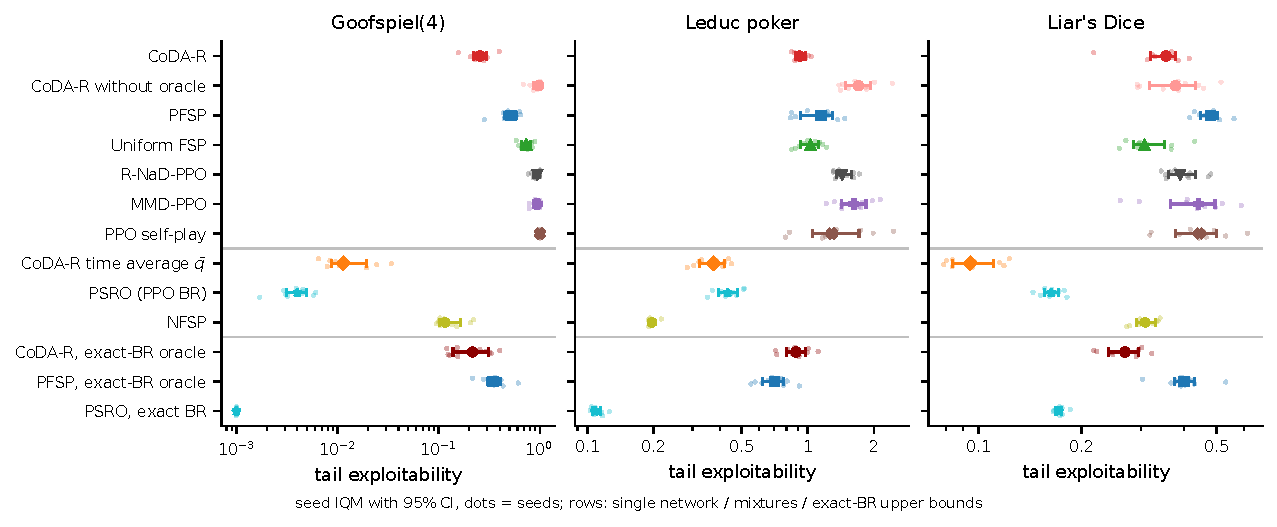
\includegraphics[width=0.9\linewidth]{figures/main_tail.pdf}
\end{center}
\caption{逐 seed 的末段 exploitability（点）及 IQM 与 95\% CI，对数坐标。各行依次为单网络、混合与精确 BR 对照。}
\label{fig:main-tail}
\end{figure}

\FloatBarrier
\subsection{大型博弈}

checkpoint 在预算比例 $1/64$、$1/16$、$1/4$、$0.8$、$0.9$ 与 $1$ 处评估（图~\ref{fig:scale}）。在与更早 checkpoint 的对局中（图~\ref{fig:scale-history}），每次运行保存 16 个 checkpoint，每个有序对进行 1000 局抽样对局并交替座位。较晚的 checkpoint 对较早的 checkpoint 的败率不超过 0.45 时，较早的 checkpoint 算作被击败；该败率不低于 0.55 时，算作它击败了较晚的 checkpoint。

\begin{figure}[!htbp]
\begin{center}
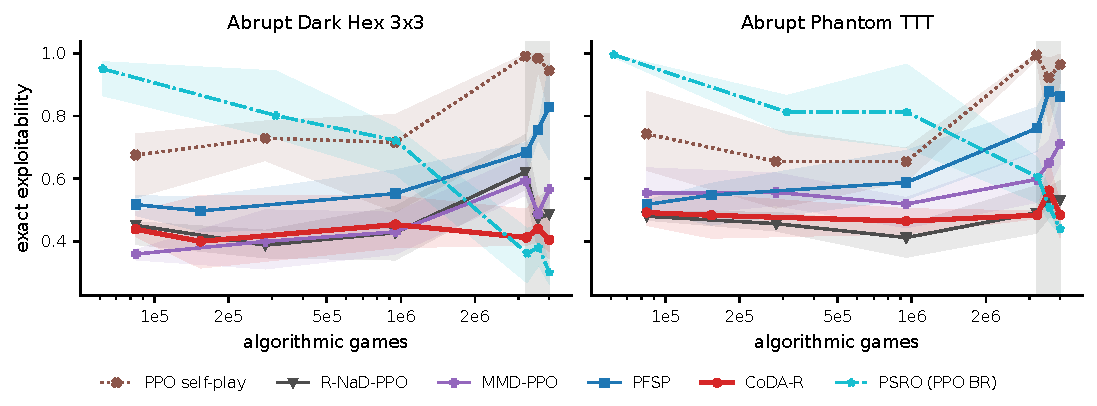
\includegraphics[width=0.85\linewidth]{figures/scale_curves.pdf}
\end{center}
\caption{大型博弈上的精确 exploitability（5 个 seed 的均值与 95\% CI）。灰带为末段。}
\label{fig:scale}
\end{figure}

\begin{figure}[!htbp]
\begin{center}
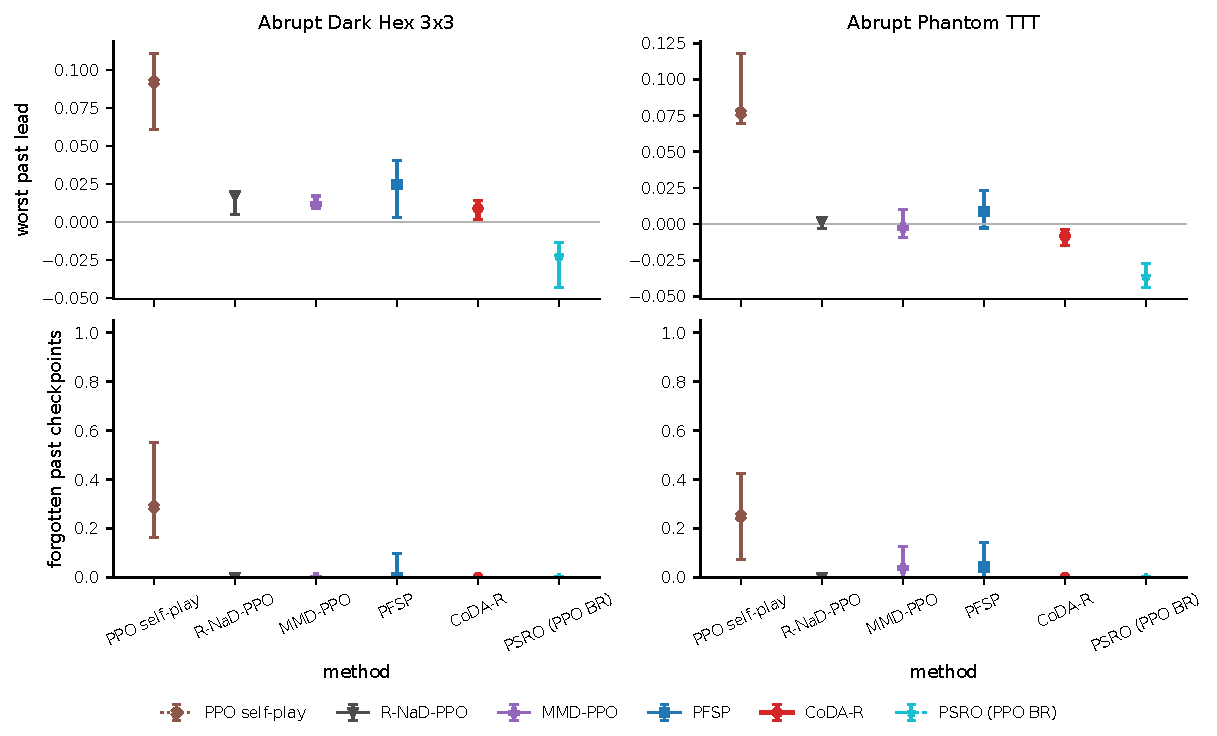
\includegraphics[width=0.85\linewidth]{figures/scale_history.pdf}
\end{center}
\caption{大型博弈上与自己更早的 checkpoint 对局。上：更早的 checkpoint 对较晚 checkpoint 的最大领先，在各 checkpoint 上平均。下：曾被击败、后来又击败了更新的 checkpoint 的 checkpoint 所占比例。}
\label{fig:scale-history}
\end{figure}

\FloatBarrier
\subsection{对手池带来什么}
\label{app:mech}

\textbf{沉睡成员。}底座网络是训练了 $2\times10^5$ 局的 \rnad{}，目标成员是它的全树最佳响应，三个诱饵是随机网络。池沿用主协议并关掉 oracle。重置之后，每个分支再训练 96 个 rollout。Hedge 与固定比例使用 \rnad{} 的 $\eta$ 与熵系数，自博弈份额为 0.5，固定比例给目标成员的系数为 0.35；移动锚规则使用 \codar{} 的配置。学习者对目标成员的败率连续 3 个 rollout 不超过 0.52 时，算作修复了它（表~\ref{tab:sleeper}、图~\ref{fig:sleeper}）。

\begin{table}[!htbp]
\caption{沉睡成员：重置后再次修复目标成员所需的 rollout 数（6 个 seed 的 IQM；“---”表示 96 个 rollout 内未修复），压制时长 $T=24/48/96/192$；以及不能击败学习者的成员所持有的训练权重份额（随 $T$ 的范围）。}
\label{tab:sleeper}
\begin{center}
\footnotesize
\setlength{\tabcolsep}{4pt}
\begin{tabular}{lcccc}
\toprule
 & \multicolumn{2}{c}{Goofspiel(4)} & \multicolumn{2}{c}{Leduc 扑克} \\
规则 & 修复时间 & 闲置权重 & 修复时间 & 闲置权重 \\
\midrule
\codar{} & 1 / 1 / 1.2 / 1 & 0.006--0.015 & 3 / 5 / 5.8 / 4.2 & 0.11--0.13 \\
移动对偶锚 & 1 / 1 / 1.2 / 1 & 0.006--0.017 & 3 / 3.7 / 4 / 3.7 & 0.17--0.22 \\
PFSP & 1 / 2.3 / 1.5 / 1.5 & 0.49--0.50 & 7.5 / 13.2 / 11 / 14.3 & 0.46--0.47 \\
Uniform FSP & 8 / 14 / 19.3 / 14.5 & 0.10 & 19.5 / 40.3 / 37.5 / 40.4 & 0.17--0.18 \\
Hedge & 0.3 / 1.7 / 4.8 / 31.5 & 0.49--0.50 & 3.3 / 8 / 9.7 / 37.7 & 0.44--0.47 \\
固定比例 & 0 / 0 / 0.2 / 0 & 0.35 & 4 / 4.7 / 5.8 / 4.3 & 0.28--0.31 \\
\rnad{}（无池） & 7.9 / 15.7 / 5.8 / 26.8 & --- & 50 / 48 / 79.5 / --- & --- \\
\bottomrule
\end{tabular}
\end{center}
\end{table}

\begin{figure}[!htbp]
\begin{center}
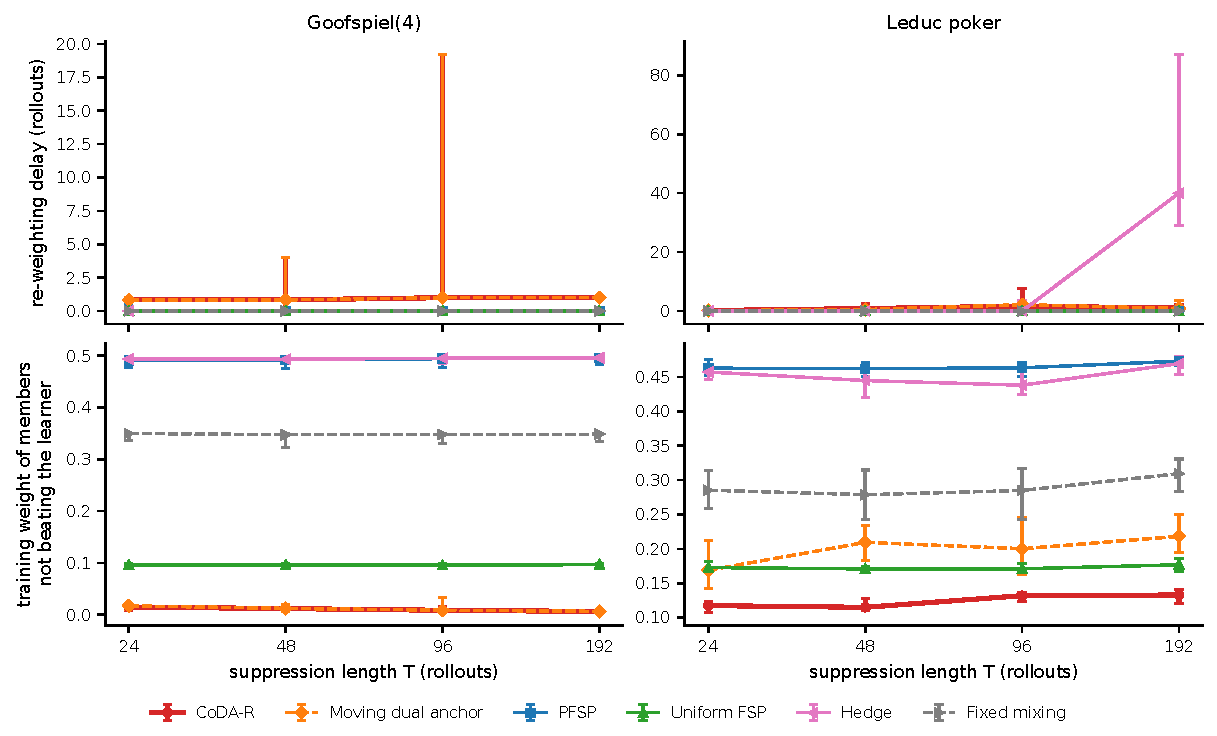
\includegraphics[width=0.8\linewidth]{figures/vuln_sleeper.pdf}
\end{center}
\caption{沉睡成员。上：目标成员拿回重置前一半系数所需的 rollout 数。下：不能击败学习者的成员所持有的训练权重份额。}
\label{fig:sleeper}
\end{figure}

\textbf{隐藏漏洞。}底座是 CFR+ 2000 次迭代的平均策略，蒸馏进与学习者同样大小的网络（每个信息集上的最大总变差为 0.006--0.028）。每一档至多埋 4 个漏洞，每个漏洞所在的信息集学习者以至少 0.1 的概率到达，且所埋动作每次到达至少损失 0.05 的归一化得分。池里只有受损网络的精确最佳响应，沿用主协议并关掉 oracle；\rnad{} 只记录它对攻击者的败率。每个分支训练 256 个 rollout，所埋动作的概率连续 3 个 rollout 不超过 0.5 时，漏洞算作被修复。Leduc 上的 $[0.3,1)$ 档作为对照，因为那里所埋的动作每次到达只损失 0.14，攻击者只领先 0.002（表~\ref{tab:hidden}）。

\begin{table}[!htbp]
\caption{隐藏漏洞：修复所需 rollout 数的中位数（6 个 seed 中修复的个数），以及攻击者的平均系数。“$>256$”表示中位数未修复。}
\label{tab:hidden}
\begin{center}
\footnotesize
\begin{tabular}{llccc}
\toprule
博弈 & 对手到达概率 & \rnad{}（无池） & PFSP & \codar{} \\
\midrule
Leduc & $[0.3,1)$（对照） & $>256$ (3) & $>256$ (2), 0.17 & $>256$ (3), 0.05 \\
Leduc & $[0.03,0.1)$ & 41.5 (6) & 19.5 (6), 0.16 & 30 (6), 0.04 \\
Leduc & $[0.003,0.01)$ & 232.5 (4) & 52 (5), 0.17 & 168.5 (4), 0.06 \\
Leduc & $[0,0.001)$ & $>256$ (0) & 8.5 (6), 0.17 & 21 (6), 0.03 \\
Goofspiel(4) & $[0.3,1)$ & 127.5 (6) & 159 (6), 0.35 & 132 (6), 0.67 \\
Goofspiel(4) & $[0,0.001)$ & $>256$ (0) & $>256$ (0), 0.05 & $>256$ (0), 0.002 \\
\bottomrule
\end{tabular}
\end{center}
\end{table}

\textbf{保持。}起始网络是同一个蒸馏的 CFR+ 底座，不埋漏洞。每种方法按主协议训练 $10^6$ 局，适用时带上各自的 oracle，熵系数固定在调参得到的最终值。exploitability 每 16 个 rollout 测量一次。归档每 128 个 rollout 收入学习者的一个副本，从底座开始；它只用于评估，对带池与不带池的方法做法相同。学习者对某个归档版本的败率不超过 0.49 时，该版本算作被击败；该败率不低于 0.51 时，算作它又击败了学习者。漂移损失是在学习者自己经常到达的信息集上，相对 CFR+ 底座的每次到达归一化得分损失，按自博弈对手到达这些信息集的概率分档（表~\ref{tab:retention}、图~\ref{fig:drift}）。

\begin{table}[!htbp]
\caption{从接近纳什的起点出发的保持情况（6 个 seed 的 IQM）：末段 exploitability 相对起点的上升，对手到达概率低于 $10^{-3}$ 一档的漂移损失，以及曾被击败、后来又击败学习者的归档版本所占比例。}
\label{tab:retention}
\begin{center}
\footnotesize
\begin{tabular}{lcccccc}
\toprule
 & \multicolumn{3}{c}{Goofspiel(4)，起点 $3.8\times10^{-4}$} & \multicolumn{3}{c}{Leduc 扑克，起点 0.0088} \\
方法 & 上升 & 漂移 & 遗忘 & 上升 & 漂移 & 遗忘 \\
\midrule
PPO 自博弈 & 1.000 & 0.0556 & 0 & 1.642 & 0.0157 & 0.229 \\
\rnad{} & 0.979 & 0.0150 & 0 & 1.353 & 0.0093 & 0 \\
MMD-PPO & 0.884 & 0.0144 & 0 & 1.316 & 0.0111 & 0.063 \\
PFSP & 0.275 & 0.0017 & 0 & 1.514 & 0.0040 & 0 \\
\codar{} & 0.135 & 0.0074 & 0 & 1.189 & 0.0030 & 0 \\
\codar{}，$c\times0.5$ & 0.177 & 0.0046 & 0 & 1.227 & 0.0029 & 0 \\
\codar{}，$c\times2$ & 0.218 & 0.0134 & 0 & 1.182 & 0.0031 & 0 \\
\bottomrule
\end{tabular}
\end{center}
\end{table}

\begin{figure}[!htbp]
\begin{center}
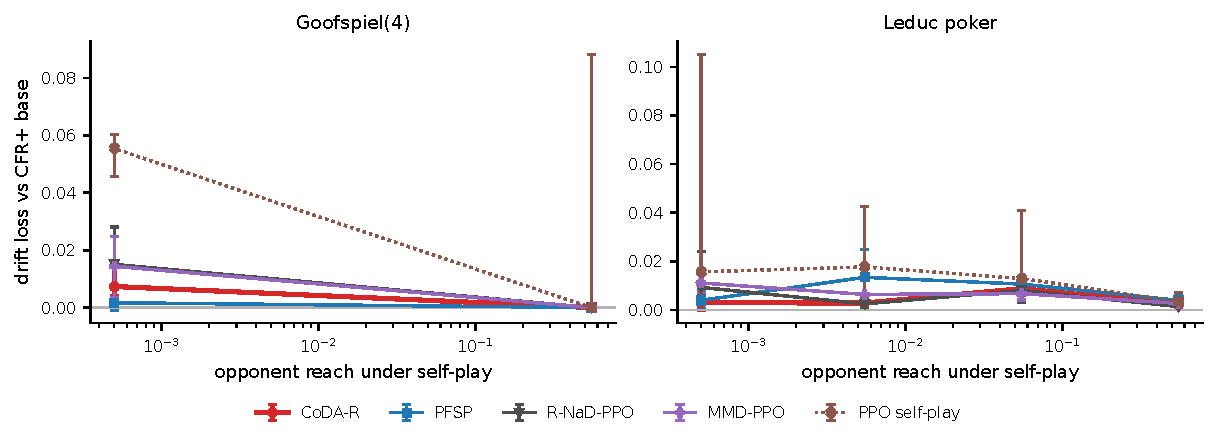
\includegraphics[width=0.8\linewidth]{figures/forgetting_drift.pdf}
\end{center}
\caption{保持：相对 CFR+ 底座的漂移损失，横轴为自博弈对手到达信息集的概率（6 个 seed 的 IQM 与 95\% CI）。在 Goofspiel(4) 上只有最高与最低两档含有信息集。}
\label{fig:drift}
\end{figure}

\textbf{开放池。}成员依次为 CFR+ 迭代 3 次与 30 次后的平均策略、两个使用 $2\times32$ 网络的旧版智能体、两个脚本对手与均匀策略，之后交替加入随机网络与重复成员，直到 $N$ 个成员。没有 oracle，也没有快照，预算为 $10^6$ 局（图~\ref{fig:open-pool}）。

\begin{figure}[!htbp]
\begin{center}
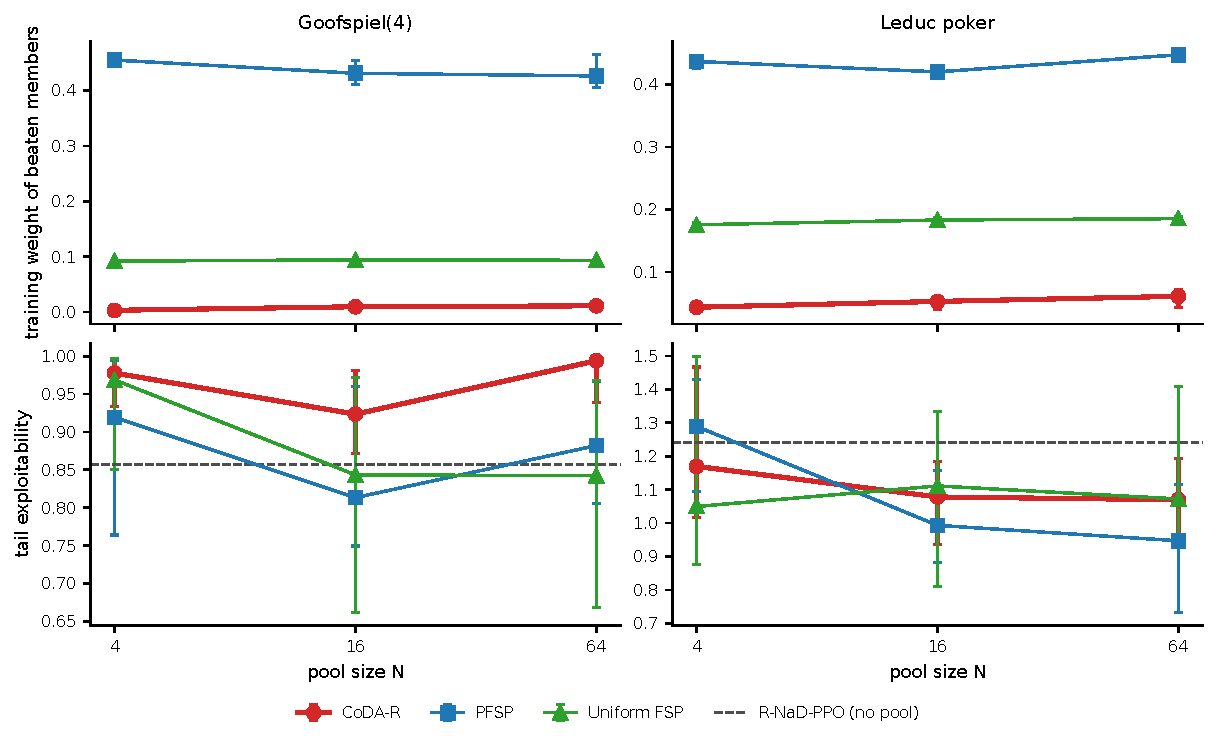
\includegraphics[width=0.8\linewidth]{figures/open_pool.pdf}
\end{center}
\caption{由 $N$ 个外部成员组成的开放池。上：学习者已经击败的成员所持有的训练权重份额。下：末段 exploitability（6 个 seed 的 IQM 与 95\% CI）；虚线为不带池的 \rnad{}。}
\label{fig:open-pool}
\end{figure}

\FloatBarrier
\subsection{消融}

在 Leduc 上，池容量 16 与基准配置相同，因为那里的池从未填满 8 个位置（图~\ref{fig:ablations}）。

\begin{figure}[!htbp]
\begin{center}
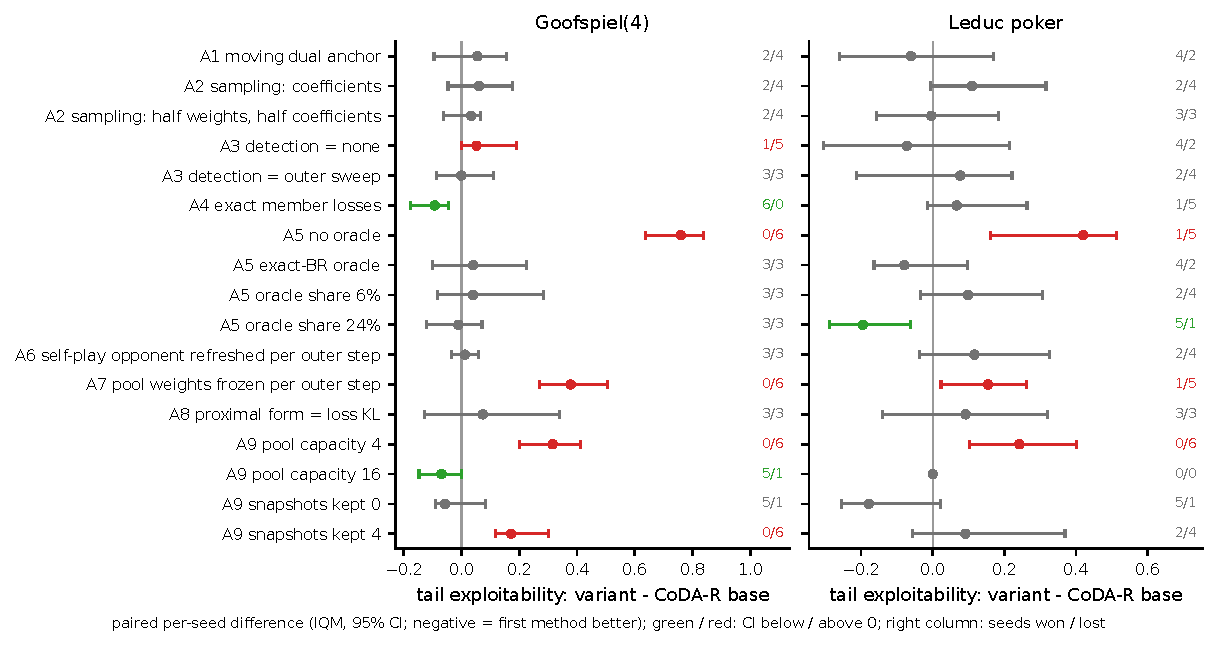
\includegraphics[width=0.9\linewidth]{figures/ablations_forest.pdf}
\end{center}
\caption{消融（$10^6$ 局，6 个 seed）：末段 exploitability 的逐 seed 配对差，变体减基准（IQM 与 95\% CI；负值更好），并标出赢与输的 seed 数。}
\label{fig:ablations}
\end{figure}

\FloatBarrier
\subsection{矩阵博弈上的精确算法}
\label{app:theory-figs}

\S\ref{sec:exp-theory} 的检查覆盖 1406 个实验格与 \S\ref{sec:theory} 的全部不等式：能量不等式、证书、速率、混合策略、注入误差 $\xi$ 与 $\delta$ 的版本，以及定理~\ref{thm:oracle}。在图~\ref{fig:oracle-rate} 中，每一步把策略锚的精确最佳响应加入池，池保留最近的 8 个成员；对偶强度为 $c=\min(4,2\eta/\|S\|^2)$，即定理~\ref{thm:oracle} 允许的最大值，近似 oracle 的误差为 $\varepsilon=0.01$。在图~\ref{fig:basin} 中，每格 200 个随机起点，博弈大小、池大小与 $\eta$ 合并统计。图~\ref{fig:adversarial} 中的对抗性池分别是周期性的最佳响应（benign）、学习者关于纳什点的反射（complement）、大量随机策略（flood）、纳什支撑上永远打平的纯策略（support），以及对很久以前的迭代的最佳响应（stale）。在图~\ref{fig:pool-rules} 中，固定份额的规则（PFSP、均匀、Hedge）停在 $10^{-2}$ 到 $6\times10^{-2}$ 之间，因为打平的成员保住了份额，而 \codar{} 与空池在重置前后都到达 $10^{-11}$。在图~\ref{fig:inexact} 中，最终 exploitability 随 $\delta$ 成比例变化，与定理~\ref{thm:inexact} 中误差有界的情形一致；估计误差只在池非空且 $\delta=0$ 时才起作用。

\begin{figure}[!htbp]
\begin{center}
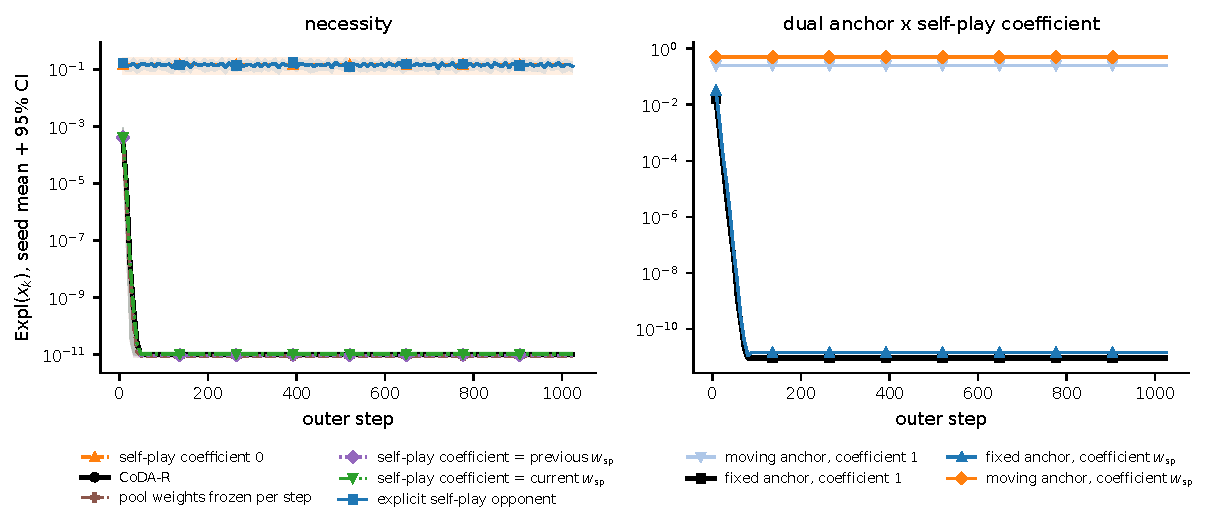
\includegraphics[width=0.85\linewidth]{figures/theory_necessity.pdf}
\end{center}
\caption{设计要素的必要性（exploitability 的 seed 均值与 95\% CI）。左：显式的自博弈对手、其他的自博弈系数，以及冻结的池权重。右：固定与移动的对偶锚，从命题~\ref{prop:rps} 的不动点出发。}
\label{fig:theory-nec}
\end{figure}

\begin{figure}[!htbp]
\begin{center}
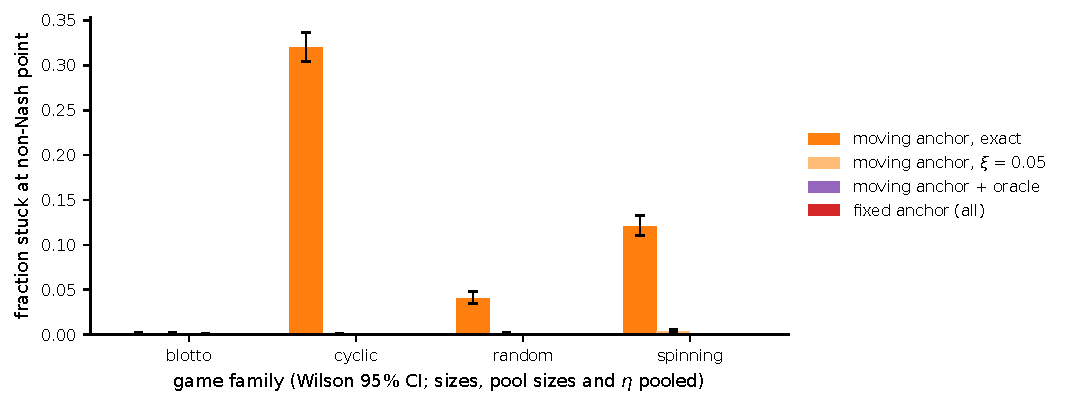
\includegraphics[width=0.75\linewidth]{figures/theory_anchor_basin.pdf}
\end{center}
\caption{移动锚卡在非纳什点上的随机起点比例（Wilson 95\% CI）。固定锚从不卡住。}
\label{fig:basin}
\end{figure}

\begin{figure}[!htbp]
\begin{center}
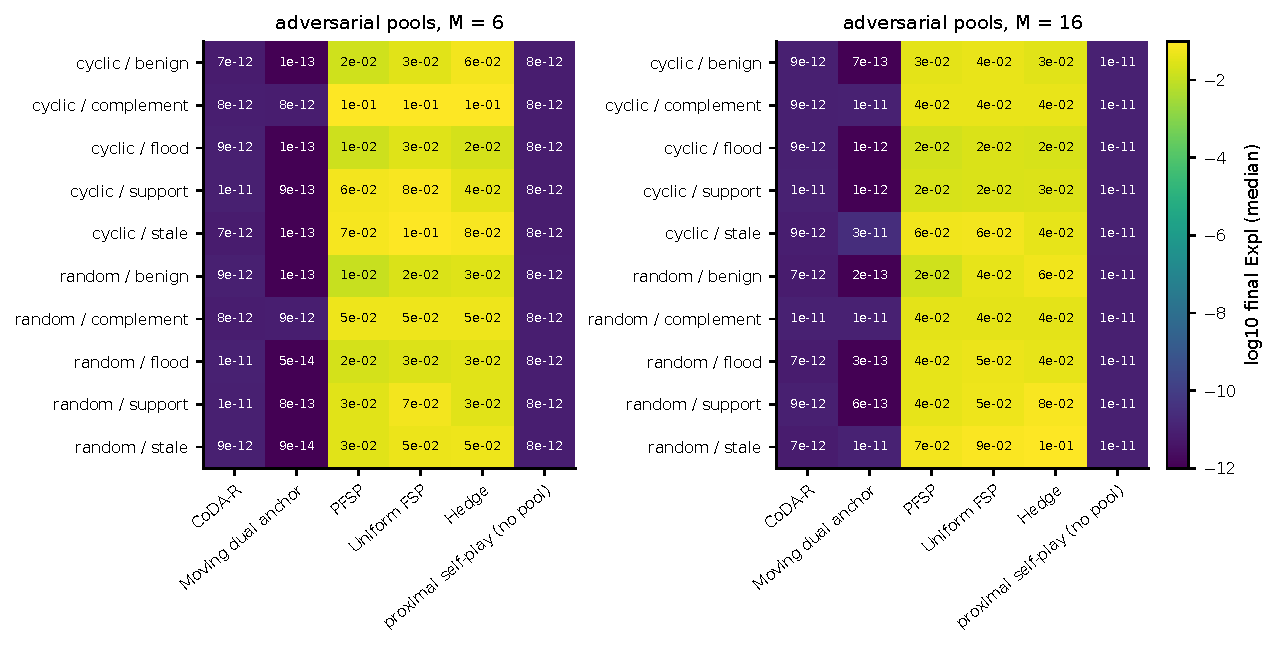
\includegraphics[width=0.9\linewidth]{figures/theory_adversarial_pool.pdf}
\end{center}
\caption{对抗性的池：由对抗者挑选池成员时，最终 exploitability 的中位数。}
\label{fig:adversarial}
\end{figure}

\begin{figure}[!htbp]
\begin{center}
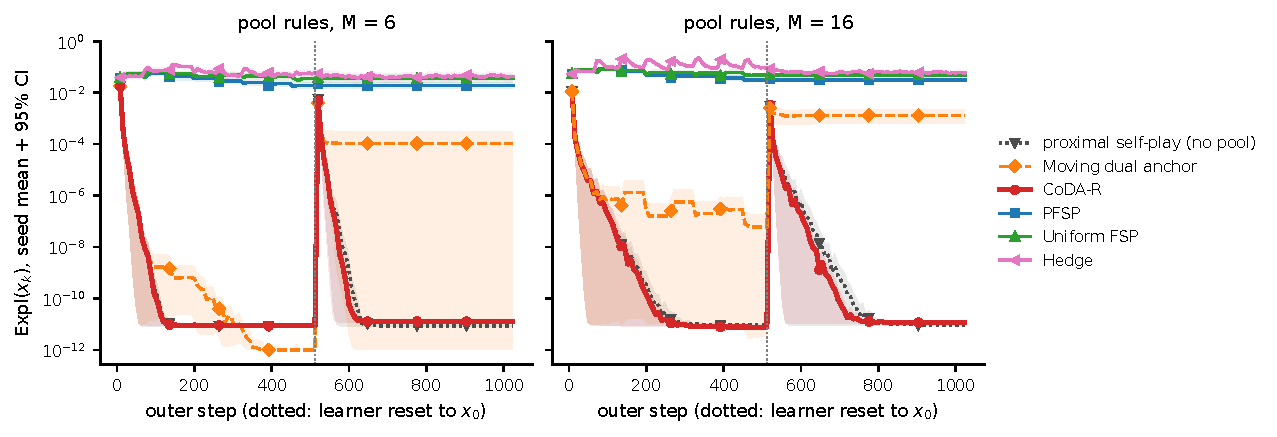
\includegraphics[width=0.9\linewidth]{figures/theory_pool_rules.pdf}
\end{center}
\caption{同一个池序列上的各种池规则；虚线处学习者被重置回初始点。}
\label{fig:pool-rules}
\end{figure}

\begin{figure}[!htbp]
\begin{center}
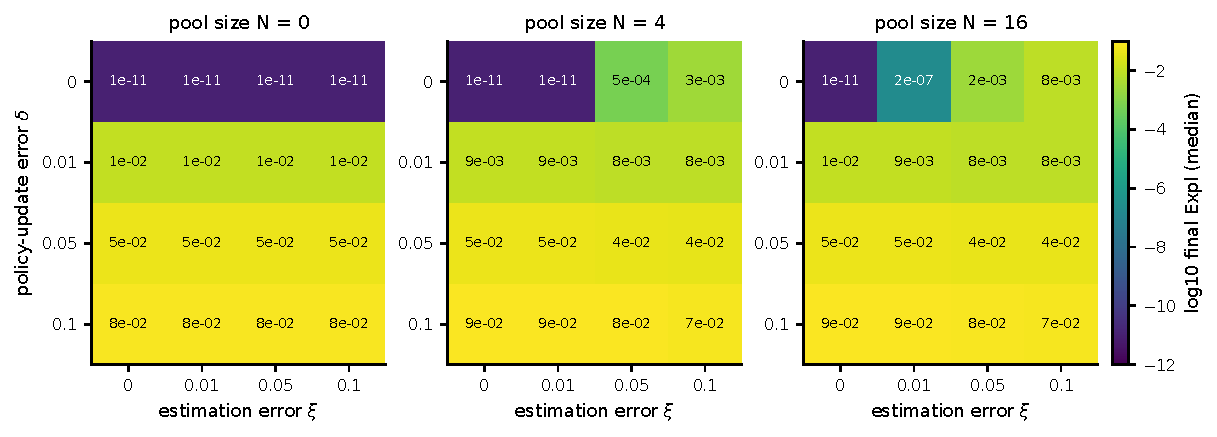
\includegraphics[width=0.85\linewidth]{figures/theory_inexact.pdf}
\end{center}
\caption{注入误差：最终 exploitability 的中位数，随估计误差 $\xi$ 与策略更新误差 $\delta$ 的变化。}
\label{fig:inexact}
\end{figure}

\end{document}

